% !TeX root = ../../thesis.tex
\chapter{Fabrication, Characterization, and Optimization of \ch{CsPbI2Br} Photodiodes}\label{ch:transport_layer}


Having established the optical, structural, and morphological properties of thermally co-evaporated \ch{CsPbI_2Br} thin films, the next step involves their integration into photodiodes for the evaluation of their optoelectronic properties. Although photodiodes designed for photovoltaic and photodetecting applications can share identical structures, differences in biasing regimes and end-use operation lead to distinct figures of merit for evaluating their performance. Both applications share the requirement for optimal absorption and extraction of the photo-generated carriers, typically quantified through the current density under illumination ($J_{photo}$) and external quantum efficiency (EQE). For photodetecting applications, the minimization of dark current ($J_d$) is of utmost importance for developing detectors with high sensitivity to signals of low intensity. On the other hand, solar cells benefit more from improvements in the open circuit voltage ($V_{oc}$), which further translate into enhanced power conversion efficiency (PCE). Nevertheless, equation $V_{oc} = \frac{nkT}{q}ln(\frac{J_{photo}}{J_{d}}+1)$, where n is the diode's ideality factor and kT/q is thermal voltage, reveals that improvements in $V_{oc}$ can be translated into lower $J_d$ and vice versa. 

The current response of a photodiode in dark conditions in the reverse bias regime is affected by multiple mechanisms which act concurrently. Specifically, $J_d$ is the sum of several current sources, including diffusion of minority carriers, thermally-activated generation-recombination, trap-assisted or band-to-band tunneling, and leakage through shunting paths. Various strategies for decreasing $J_d$ have been investigated, such as the promotion of perovskites with larger grains for the elimination of shunt pathways \cite{Jang2022PreventionPhotodetection, Yang2024High-PerformancePathways}, the annihilation of bulk defects for the restriction of trap-assisted tunneling \cite{Furlan2022TuningDetectivity, Yao2019High-Rubidium-Formamidinium-RatioStability, Li2020Self-poweredStability}, and lastly the increment of the interfacial energy offset between the perovskite and charge transport layers to suppress interfacial thermal charge generation \cite{Ollearo2021UltralowGeneration, Martinez-Goyeneche2024Vacuum-DepositedDetection, Ollearo2022MultidimensionalPhotodiodes}. 

Nonetheless, most of the aforementioned studies limit their operational voltage range to -0.5 V, as higher reverse biases exacerbate tunneling effects and increase the risk of reverse-bias breakdown. This is in contrast to our intended application, which requires reliable operation up until, at least, -2 V for reasons described in Section~\ref{sec:scope_and_aim}. In this chapter we detail our efforts to develop efficient and reliable all-inorganic, vacuum-deposited PePDs. Beginning with the fabrication of bottom-illuminated photodiodes on transparent substrates, we investigate the impact of perovskite deposition conditions and the choice of ETL. The latter proves critical to both device reliability and response speed. Subsequently, the optimized stack is transferred to silicon substrates for the characterization of the top-illuminated configuration, with special emphasis given on its high-temperature tolerance.


\section{Development of Bottom-Illuminated PePDs}

\subsection{Benchmarking Performance}

Previous work, conducted within the group, evaluated the use of the \ch{CsPbI_3} perovskite as the active layer in all-inorganic photodiodes \cite{PintorMonroy2021All-EvaporatedApplications}. The study relied on the use of DC sputtered \ch{NiO_x} as the HTL and e-beam evaporated \ch{TiO_2} as the ETL in a p-i-n  device architecture. Building upon this study, we start by evaluating the use of the \ch{CsPbI_2Br} composition in the same device stack. A key distinction between the two materials lies in their initial phase composition. The as-deposited \ch{CsPbI_3} perovskite appears in a "brown" phase, which is a mixture of the $\delta$- and $\gamma$-phases. As a result, a post-deposition annealing step at 320 \degree C is required to isolate the pure $\gamma$-phase. In contrast, our analysis in Chapter~\ref{ch:ellipsometry} revealed that the as-deposited \ch{CsPbI_2Br} composition already crystallizes in the $\gamma$-phase, making the post-deposition thermal annealing step not strictly necessary. 

\begin{figure}[htbp]
    \centering
    % First row
    \begin{subfigure}[t]{0.32\textwidth}
        \centering
        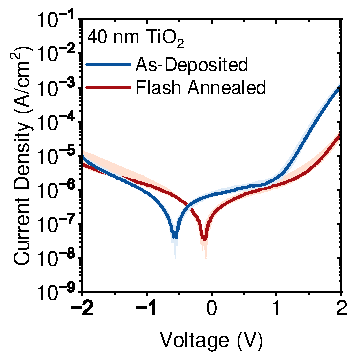
\includegraphics[width=\textwidth]{chapters/material_properties/images/TiO2-Compare.pdf} 
        \caption{}
        \label{fig:ch2:tio2_compare}
    \end{subfigure}
    \hfill
    \begin{subfigure}[t]{0.32\textwidth}
        \centering
        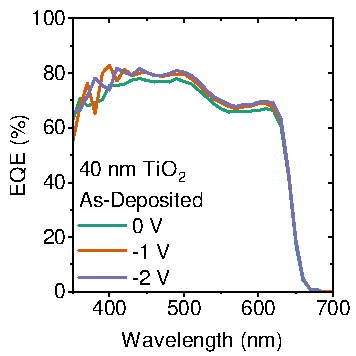
\includegraphics[width=\textwidth]{chapters/material_properties/images/As_Dep-EQE.pdf} % Replace with your image file
        \caption{}
        \label{fig:ch2:as_dep_eqe}
    \end{subfigure}
    \hfill
    \begin{subfigure}[t]{0.32\textwidth}
        \centering
        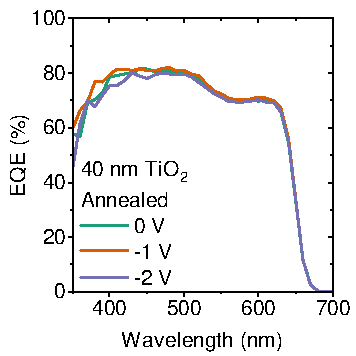
\includegraphics[width=\textwidth]{chapters/material_properties/images/Annealed_EQE.pdf} % Replace with your image file
        \caption{}
        \label{fig:ch2:annealed_eqe}
    \end{subfigure}
    \caption[Impact of thermal annealing on JVs and EQE of PePDs with 40 nm of \ch{TiO_2} as the ETL.]{(a) Comparison of current density as a function of bias for two PePDs with an as-deposited and flash-annealed perovskite layer, both featuring a 40 nm \ch{TiO_2} ETL. EQE as a function of wavelength under steps of increasing reverse bias for a PePD with an (b) as-deposited and (c) flash annealed perovskite layer.}
    \label{fig:ETL_opt:annealing_impact}
\end{figure}

As a result, we start our investigation by comparing the photodiode performance of two stack variations: one utilizing an as-deposited \ch{CsPbI_2Br} layer and the other incorporating a flash-annealed perovskite at 300 \degree C in a \ch{N_2} environment. Results indicate that the flash-annealed devices exhibit only slightly lower levels of median $J_d$ at -2 V (9.5 $\mu A/cm^2$ for the as-deposited and 6 $\mu A/cm^2$ for the annealed perovskite), as shown in Figure~\ref{fig:ETL_opt:annealing_impact}a. Additionally, their EQE response is almost identical, already saturated at 0 V and beyond 70\% across most of the visible light spectrum (Figure~\ref{fig:ETL_opt:annealing_impact}b,c). These results reveal that the improvements in film quality achieved through thermal annealing, including higher crystallinity and fewer non-radiative recombination pathways as discussed in Chapter~\ref{ch:ellipsometry}, are not directly translated to improvements in device performance, at least in terms of $J_d$ and EQE. Even though the use of as-deposited perovskites is highly relevant for alternative applications that require low-temperature processing (such as the fabrication of PePDs on flexible substrates), the rest of the presented results in this thesis rely on the flash annealing of the perovskite layer at 300 \degree C in \ch{N_2} environment before the deposition of the ETL. 


Besides its annealing conditions, additional parameters of the perovskite layer that can be tuned include its CsBr to \ch{PbI_2} molar ratio, as well as the total deposition rate. It is reminded that the results presented earlier were based on a 1.05:1.0 CsBr:\ch{PbI_2} molar ratio and a 0.8 \AA/s deposition rate. 

\begin{figure}[htbp]
    \centering
    
    % Second row
    \begin{subfigure}[t]{0.45\textwidth}
        \centering
        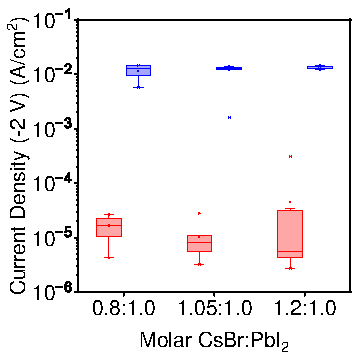
\includegraphics[width=\textwidth]{chapters/transport_layers/images/JV_Box_Ratio.pdf} % Replace with your image file
        \caption{}
        \label{fig:etl_opt:molar_ratio}
    \end{subfigure}
    \hfill
        \begin{subfigure}[t]{0.45\textwidth}
        \centering
        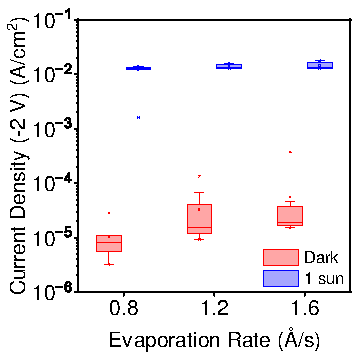
\includegraphics[width=\textwidth]{chapters/transport_layers/images/Evap_Rate_Box_Plot.pdf} % Replace with your image file
        \caption{}
        \label{fig:etl:opt:evap_rate}
    \end{subfigure}    
    \caption[Impact of CsBr to \ch{PbI_2} molar ratio and total evaporation rate during the perovskite deposition on current density of the PePDs with 40 nm of \ch{TiO_2} as the ETL.]{(a) Statistical results of current density at -2 V in dark and under 1-sun illumination for PePDs featuring a perovskite layer with 0.8:1.0, 1.05:1.0, and 1.2:1.0 CsBr-to-\ch{PbI_2} molar ratio. (b) Statistical results of current density at -2 V in dark and under 1-sun illumination for PePDs featuring a perovskite layer deposited with 0.8, 1.2 an 1.6 \AA/s total deposition rate. }
    \label{fig:etl_opt:molar_and_rate}
\end{figure}

In terms of varying the precursor molar ratio, we explored two additional compositions, a \ch{PbI_2}-rich (\ch{CsBr}:\ch{PbI_2} = 0.8:1.0) and a \ch{CsBr}-rich (\ch{CsBr}:\ch{PbI_2} = 1.2:1.0) one. The respective results, displaying the variation of $J_d$ and $J_{photo}$ at -2 V for each condition, are shown in Figure~\ref{fig:etl_opt:molar_and_rate}a. The median $J_{photo}$ at -2 V was approximately equal to 13 $mA/cm^2$ for all compositions, while the median $J_d$ varied between 5.5 and 16 $\mu A/cm^2$. The 1.05:1.00 composition exhibited the optimal balance of the lowest $J_d$ values and reduced device-to-device variability, even though increasing the amount of CsBr in the film seemed to have a positive effect on the median $J_d$ response. Nevertheless, the difference in performance among devices with different stoichiometry remains relatively small, highlighting the defect tolerance of the perovskite thin films. This means that deviations from the 1.0:1.0 stoichiometry and consequent formation of defects or vacancies does not necessarily lead to increased levels of dark current. Therefore, the potential defect states likely have shallow energy levels that do not promote trap-assisted charge carrier generation in dark conditions.


For the evaluation of the impact of the total evaporation rate, the nominal 1.05:1.0 \ch{CsBr}:\ch{PbI_2} ratio was maintained, with the evaporation rate was varied between 0.8 and 1.6 \AA/s. Increasing the total deposition rate would be relevant for speeding up the fabrication process and increasing experimental throughput. Additionally, the evaporation rate, along with the substrate temperature, is one of the most critical parameters for the nucleation of the perovskite thin film, as described by equation: 

\begin{equation}
    N \propto \frac{F^p}{D^q}, 
\end{equation}

where N is nuclear density, F is the evaporation rate, and D is the surface diffusion coefficient \cite{Dong2023GrowthFilm}. The values $p$ and $q$ are positive and depend on the nucleation and growth mechanisms. As a result, higher evaporation rates are typically associated with the attainment of smaller grain sizes \cite{Dong2023GrowthFilm, Du2022ThermalOutlook, Shin2020ModulationDiodes}. Increasing the deposition rate of our thermally evaporated \ch{CsPbI_2Br} thin films from 0.8 \AA/s to 1.6 \AA/s leads to an increase of the median $J_d$ at -2 V from 8 $\mu A/cm^2$ to 19 $\mu A/cm^2$, while the the median $J_{photo}$ is maintained at approximately  13 $\mu A/cm^2$ (Figure~\ref{fig:etl_opt:molar_and_rate}a). This finding prevents us from adopting a faster deposition rate in favor of a higher experimental throughout. Consequently, a total deposition rate of 0.8 \AA/s is maintained for the remainder of the presented results. 




The results presented thus far provide an initial benchmark for PePD performance and examine the impact of various perovskite-processing parameters. While certain variations are observed, especially in the levels of $J_d$, the impact of the thermal annealing, precursors ratio and total evaporation rate remains rather low, highlighting the overall high quality and defect tolerance of the \ch{CsPbI_2Br} thin films. 

\begin{figure}[htbp]
    \centering
    % Second row
    \begin{subfigure}[t]{0.5\textwidth}
        \centering
        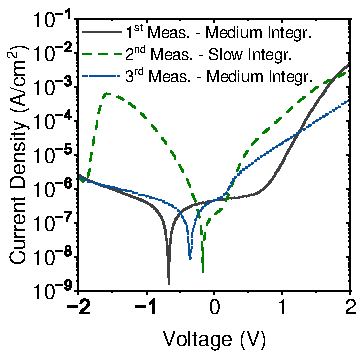
\includegraphics[width=\textwidth]{chapters/transport_layers/images/JV_TiO12_Scan_Speed.pdf} % Replace with your image file
                
    \end{subfigure}

    \caption[Impact of scan integration time on the J–V characteristics of a PePD with a 40 nm \ch{TiO_2} ETL.]{Impact of scan integration time on the J–V characteristics of a PePD with a 40 nm \ch{TiO_2} ETL. The sharp increase in current density under reverse bias during the slow integration scan is an indication of a breaking down mechanism, which, however, is non-destructive as confirmed by the repeated J–V scan using a medium integration time.}
    \label{fig:tio2:scan_speed}
\end{figure}

However, an interesting feature comes across when trying to characterize the performance of the baseline PePD in dark conditions using different integration times during the J-V scan. There results are presented in Figure~\ref{fig:tio2:scan_speed}, where the standard J-V scan with medium integration time is followed by a scan with slow integration time. Even though both measurements start from similar $J_d$ levels, the scan with slow integration time displays an abrupt, almost 3-order of magnitude, increase in the $J_d$ levels while the diode still in the reverse bias regime. The reversibility of this phenomenon is demonstrated by repeating the J–V scan with a medium integration time, during which the original performance is restored. This pattern indicates the triggering of a non-destructive reverse-bias breakdown mechanism, which depends not only on the magnitude of the applied reverse bias, but also its duration \cite{Bertoluzzi2021IncorporatingBias}. Such phenomena have previously been studied in the context of shaded perovskite solar cells, which must carry the current generated by adjacent illuminated cells \cite{Jiang2024ImprovedElectrodes, Ren2024MobileCells, Li2024BarrierBias,Gould2021In-OperandoBias,Razera2020InstabilityBias,Bertoluzzi2021IncorporatingBias,Wang2023PerovskiteDegradation,Bowring2018ReverseCells, Ni2021EvolutionIllumination}. Specifically, it was shown that under reverse bias ions accumulate at the perovskite/ETL interface, facilitating the tunneling of holes into the perovskite bulk due to increased band-bending. Recombination centers are thereafter generated by the oxidation of halides to natural halogens \cite{Bertoluzzi2021IncorporatingBias}. Diffusion of iodine into the fullerene-based ETL was also shown to be an aftermath of reverse biasing \cite{Razera2020InstabilityBias}. Various breakdown mitigation strategies were proposed, including the introduction of a hole-blocking layer at the perovskite/ETL interface, the use of electrochemically inert electrodes, as well as the deposition of a thick planarizing polymer HTL. However, reverse-bias breakdown has not been considered in the context of PePDs, where reverse biasing is the standard operating condition. The following section provides a detailed analysis of the reverse-bias breakdown in our vacuum-deposited, all-inorganic PePDs, with a particular focus on the influence of the ETL/perovskite interface quality.


\subsection{Enhancement of Reverse Bias Stability}

\begin{figure}[htbp]
    \centering
    \begin{subfigure}{0.24\textwidth}
        \centering
        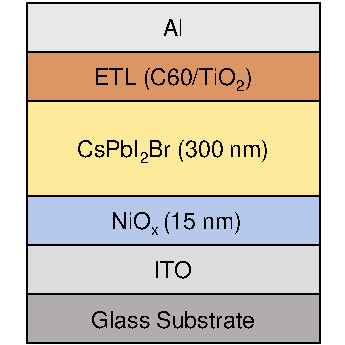
\includegraphics[width=\textwidth]{chapters/transport_layers/images/ETL_optimization_stack.pdf}
        \caption{}
        \label{}
    \end{subfigure}
    \hfill
    \begin{subfigure}{0.24\textwidth}
        \centering
        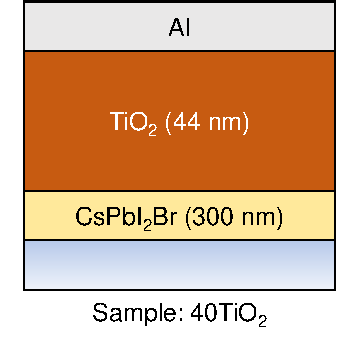
\includegraphics[width=\textwidth]{chapters/transport_layers/images/ETL_Optimization_40TiO2.pdf}
        \caption{}
        \label{}
    \end{subfigure}
    \hfill
    \begin{subfigure}{0.24\textwidth}
        \centering
        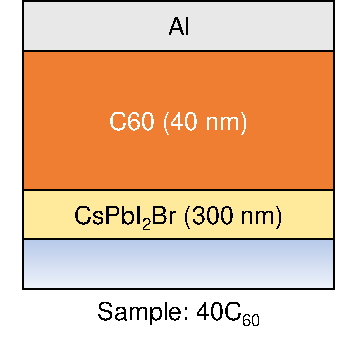
\includegraphics[width=\textwidth]{chapters/transport_layers/images/ETL_Optimization_40C60.pdf}
        \caption{}
        \label{}
    \end{subfigure}
    \hfill
    \begin{subfigure}{0.24\textwidth}
        \centering
        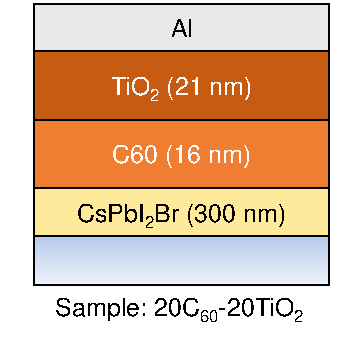
\includegraphics[width=\textwidth]{chapters/transport_layers/images/ETL_Optimization_20_20.pdf}
        \caption{}
        \label{}
    \end{subfigure}
    
    \caption[Schematic illustration of ETL combinations used in this study.]{(a) Schematic illustration of the bottom illuminated PePD. Variations of the ETL combinations used in this study, including (b) a single 40 nm \ch{TiO_2} layer, (c) a single 40 nm \ch{c_{60}} layer, and (d) a \ch{C_{60}} – \ch{TiO_2} bilayer, each 20 nm thick.}
    \label{fig:etl_optimization:stacks}
\end{figure}

Considering the importance of the ETL choice on the reverse-bias stability of perovskite-based diodes, we fabricated three variation of the same stack, employing 40 nm of \ch{TiO_2} (Sample 40\ch{TiO_2}), 40 nm of \ch{C_{60}} (Sample 40\ch{C_{60}}), and a 40 nm of a \ch{C_{60}}-\ch{TiO_2} bilayer (Sample 20\ch{C_{60}}-20\ch{TiO_2}) as the device's ETL, as shown in Figure~\ref{fig:etl_optimization:stacks}a-d. \ch{C_{60}} is considered as an alternative ETL in this study given its compatibility with vacuum deposition processes and its demonstrated thermal stability at temperatures exceeding 250 \degree C \cite{Sundar1992ThermalC60, Bracesco2024InPhotovoltaics}. In most cases, a buffer layer, such as bathocuproine (BCP) or lithium fluoride (LiF), is introduced above or below the \ch{C_{60}} layer to mitigate charge buildup and minimize non-radiative recombination losses \cite{Chen2017EffectCells, Ye2022OvercomingCarborane}. However, both materials have been linked with reducing a device's operational and thermal stability, which is why they were deliberately excluded from this study \cite{Al-Ashouri2020MonolithicExtraction, Zheng2020EnhancedStrategy}. Figure~\ref{fig:etl_optimization:eds_tem_crossection}a and b displays the scanning transmission electron microscopy (STEM) high-angle annular dark-field imaging (HAADF) cross-section of samples 40\ch{TiO_2} and 40\ch{C_{60}}, superimposed with their energy dispersive X-Ray spectroscopy (EDS) elemental mapping. All layers appear continuous and compact, with no visible pinholes, cracks, or defects. Based on EDS measurements, the perovskite composition is estimated to be \ch{Cs_{1.15}PbI_{1.83}Br_{1.24}} for both samples.


\begin{figure}[ht!]
    \centering
    % First plot
    \begin{subfigure}[t]{0.45\textwidth} % Adjust width as needed
        \centering
        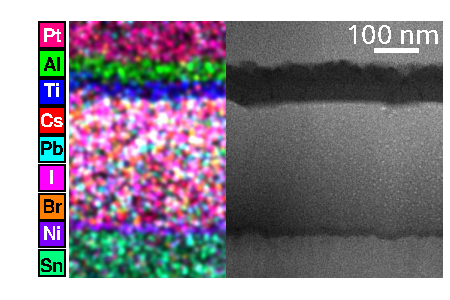
\includegraphics[width=\textwidth]{chapters/transport_layers/images/EDS_TEM_TiO2.pdf} % Replace with your image
        \caption{}
        \label{}
    \end{subfigure}
    \hfill % Space between the two plots
    % Second plot
    \begin{subfigure}[t]{0.45\textwidth} % Adjust width as needed
        \centering
        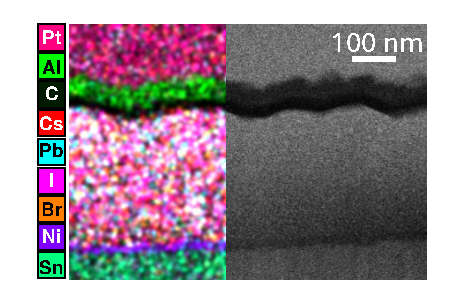
\includegraphics[width=\textwidth]{chapters/transport_layers/images/EDS_TEM_C60.pdf} % Replace with your image
        \caption{}
        \label{}
    \end{subfigure}
    % Caption for the whole figure
    \caption[STEM-HAADF and EDS elemental map of the 40\ch{TiO_2} and 40\ch{C_{60}} samples.]{STEM-HAADF image of the (a) 40\ch{TiO_2} and (b) 40\ch{C_{60}} samples, both superimposed with the respective EDS elemental map.}
    \label{fig:etl_optimization:eds_tem_crossection}
\end{figure}

\begin{figure}[ht!]
    \centering

    % First row
    \begin{subfigure}[b]{0.32\textwidth}
        \centering
        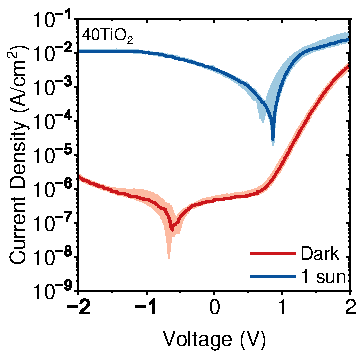
\includegraphics[width=\textwidth]{chapters/transport_layers/images/JV_Median_40TiO2.pdf}
        \caption{}
    \end{subfigure}
    \hfill
    \begin{subfigure}[b]{0.32\textwidth}
        \centering
        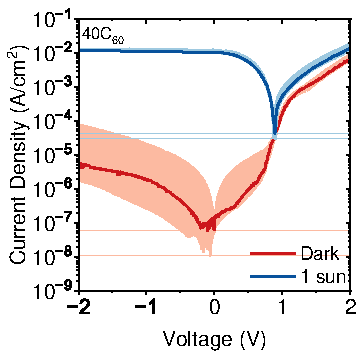
\includegraphics[width=\textwidth]{chapters/transport_layers/images/JV_Median_40C60.pdf}
        \caption{}
    \end{subfigure}
    \hfill
    \begin{subfigure}[b]{0.32\textwidth}
        \centering
        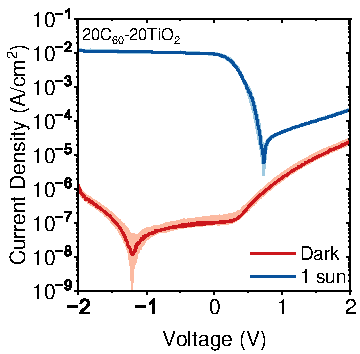
\includegraphics[width=\textwidth]{chapters/transport_layers/images/JV_Median_20_20.pdf}
        \caption{}
    \end{subfigure}


        \begin{subfigure}{0.32\textwidth}
        \centering
        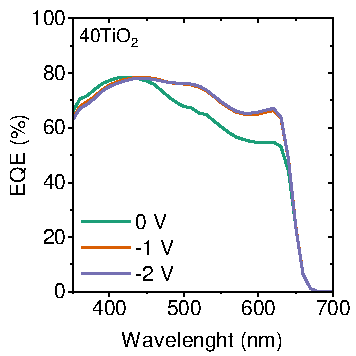
\includegraphics[width=\textwidth]{chapters/transport_layers/images/EQE_40TiO2.pdf}
        \caption{}
        \label{}
    \end{subfigure}
    \hfill
    \begin{subfigure}{0.32\textwidth}
        \centering
        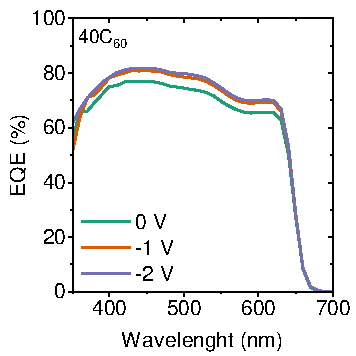
\includegraphics[width=\textwidth]{chapters/transport_layers/images/EQE_40C60.pdf}
        \caption{}
        \label{}
    \end{subfigure}
    \hfill
    \begin{subfigure}{0.32\textwidth}
        \centering
        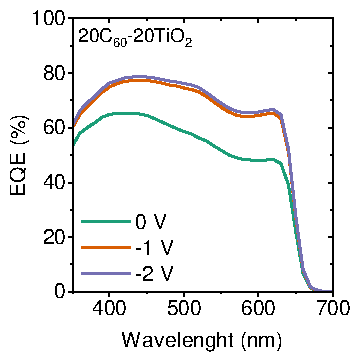
\includegraphics[width=\textwidth]{chapters/transport_layers/images/EQE_20_20.pdf}
        \caption{}
        \label{}
    \end{subfigure}

    % Second row
    \begin{subfigure}[b]{0.32\textwidth}
        \centering
        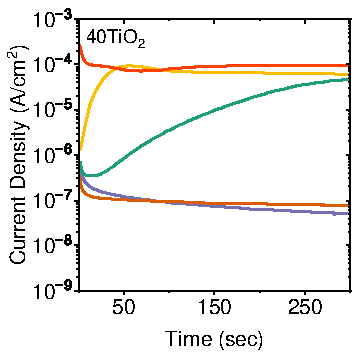
\includegraphics[width=\textwidth]{chapters/transport_layers/images/StaticJV_40TiO2.pdf}
        \caption{}
    \end{subfigure}
    \hfill
    \begin{subfigure}[b]{0.32\textwidth}
        \centering
        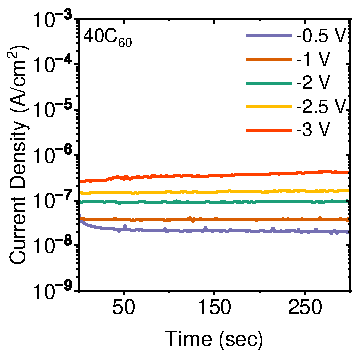
\includegraphics[width=\textwidth]{chapters/transport_layers/images/StaticJV_40C60.pdf}
        \caption{}
    \end{subfigure}
    \hfill
    \begin{subfigure}[b]{0.32\textwidth}
        \centering
        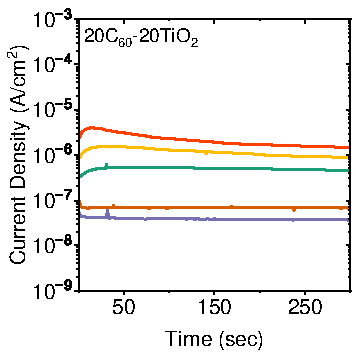
\includegraphics[width=\textwidth]{chapters/transport_layers/images/StaticJV_20_20.pdf}
        \caption{}
    \end{subfigure}

    \caption[Overview of electrical characterization results for PePDs with 40 nm of \ch{TiO_2}, 40 nm of \ch{C_{60}}, or  20 nm of \ch{C_{60}} and 20 nm of \ch{TiO_2} as the ETL.]{Current density as a function of bias in dark and under 1-sun illumination for samples (a) 40\ch{TiO_2}, (b) 40\ch{C_{60}}, and (c) 20\ch{C_{60}}-20\ch{TiO_2}. EQE as a function of wavelength under steps of increasing reverse bias for samples (d) 40\ch{TiO_2}, (e) 40\ch{C_{60}}, and (f) 20\ch{C_{60}}-20\ch{TiO_2}. Steady state measurements of current density as a function of time in dark under steps of increasing reverse bias for samples (g) 40\ch{TiO_2}, (h) 40\ch{C_{60}}, and (i) 20\ch{C_{60}}-20\ch{TiO_2}. An additional 300~s recovery period in dark conditions was implemented between two consecutive measurements.}
    \label{fig:etl_opt:dynamicjv_eqe_staticjv}
\end{figure}

Figure~\ref{fig:etl_opt:dynamicjv_eqe_staticjv}a-i provide a complete overview of the PePD performance for the three stack variations. Specifically, Figure~\ref{fig:etl_opt:dynamicjv_eqe_staticjv}a-c show the dynamic J-V scan in darkness and under 1 sun illumination, Figure~\ref{fig:etl_opt:dynamicjv_eqe_staticjv}d-f show the spectral EQE response of a single device, and lastly Figure~\ref{fig:etl_opt:dynamicjv_eqe_staticjv}g-i show the static $J_d$ measurements as function of time for increasing reverse bias steps. After each measurement, each device was given an additional 300 seconds to reset in dark. Figure~\ref{fig:etl_opt:dynamicjv_eqe_staticjv}g highlights the sensitivity of 40\ch{TiO_2} sample to reverse bias breakdown, which is not hinted by the dynamic scan of Figure~\ref{fig:etl_opt:dynamicjv_eqe_staticjv}a. In more detail, $J_d$ is maintained below 0.1 $\mu A/cm^2$ after the end of the static scan at -0.5 and -1 V, however, a 3-order of magnitude increase is observed once the bias surpasses -2 V. It is important to emphasize that the primary objective of the work presented in this thesis is geared toward imager applications, where the PePDs operate under reverse bias conditions for sub-second durations during signal integration. The duration of this read-out cycle might not be sufficient for the manifestation of the $J_d$ increase, nonetheless, this bias sensitivity could be detrimental for alternative applications that require extensive reverse biasing. Additionally, the observed breakdown mechanism also points to the presence of a defective stack, which could affect device performance in unforeseen ways. Therefore, it is essential to further investigate and address this issue.


\begin{figure}[htbp]
    \centering
    % Second row
    \begin{subfigure}[t]{0.5\textwidth}
        \centering
        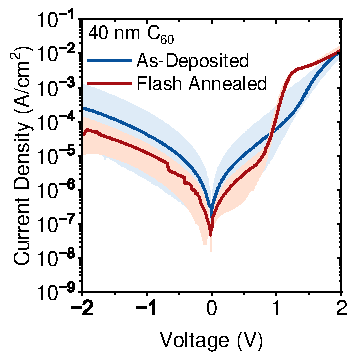
\includegraphics[width=\textwidth]{chapters/material_properties/images/C60-Compare.pdf} % Replace with your image file
                
    \end{subfigure}

    \caption[Impact of perovskite annealing on the median current density and interquartile range in dark conditions for PePDs that feature a 40 nm \ch{C_{60}} layer.]{Impact of perovskite annealing on the median current density and interquartile range in dark conditions for PePDs that feature a 40 nm \ch{C_{60}} layer.}
    \label{fig:et_optim:c60_variability}
\end{figure}

\begin{figure}[htbp]
    \centering
    % Second row
    \begin{subfigure}[t]{0.5\textwidth}
        \centering
        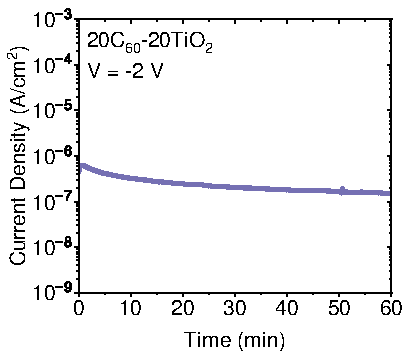
\includegraphics[width=\textwidth]{chapters/transport_layers/images/JV_1hr_20_20.pdf} % Replace with your image file
                
    \end{subfigure}

    \caption[Current density as a function of time for sample 20\ch{TiO_2}-20\ch{C_{60}} under prolonged (1 hr) biasing at -2 V.]{Current density as a function of time for sample 20\ch{TiO_2}-20\ch{C_{60}} under prolonged (1 hr) biasing at -2 V. No sings of breakdown are observed with the specific stack configuration.}
    \label{fig:et_optim:1hr_stability}
\end{figure}


In contrary to sample 40\ch{TiO_2}, the static $J_d$ scan of sample 40\ch{C_{60}} (Figure~\ref{fig:etl_opt:dynamicjv_eqe_staticjv}h) shows an almost linear increase of $J_d$ as a function of applied reverse bias, with no indications of breaking down up to -3 V. This result further strengthens the assumption that the perovskite/ETL interface is one of the most critical factors for the reverse bias stability of a PePD. Despite the improved bias stability, sample 40\ch{C_{60}} is also associated with a large variability in device performance, as indicated by the spread of the interquartile range in Figure~\ref{fig:etl_opt:dynamicjv_eqe_staticjv}b. The fact that this variability is only observed for the 40\ch{C_{60}} sample is likely due to the incomplete coverage of the perovskite film by the \ch{C_{60}} layer, which leads to the formation of contact pathways between the metal conductor and the perovskite layer \cite{Lin2015LowImaging, Younes2021EnhancingLayer}. This phenomenon seems to be aggravated by the perovskite's small grain size and large amount of grain boundaries, as indicated by the comparison of the J-V performance of two PePDs that employ an as-deposited and flash annealed \ch{CsPbI_2Br} thin film in Figure~\ref{fig:et_optim:c60_variability}). Specifically, both the median $J_d$ and the interquartile range show improvement with annealing of the perovskite layer. Nevertheless, the variability of the annealed 40\ch{C_{60}} sample is still significant and unsuitable for a reliable PePD. 




Considering that \ch{C_{60}} is preventing the reverse bias breakdown of the PePD and the use of \ch{TiO_2} ensures higher performance repeatability, the use of a \ch{C_{60}}-\ch{TiO_2} bilayer (of 20 nm each) effectively secures both advantages, as revealed in Figure~\ref{fig:etl_opt:dynamicjv_eqe_staticjv}c and i. Specifically, $J_d$ remains below 0.5 $\mu A/cm^2$ when the device is biased at -2 V for 300 s and below 2 $\mu A/cm^2$ when biased at -3 V for the same duration. Additionally, there are no signs of breakdown even when biasing the device for 60 minutes at -2 V (Figure~\ref{fig:et_optim:1hr_stability}). Finally, even though a slightly lower EQE at 0 V is observed compared to samples 40\ch{TiO_2} and 40\ch{C_{60}} (Figure~\ref{fig:etl_opt:dynamicjv_eqe_staticjv}f), a saturated efficiency, above 70\% across the entire visible range, is attained at -1 and -2 V. 

\begin{figure}[htbp]
    \centering
    \begin{subfigure}{0.32\textwidth}
        \centering
        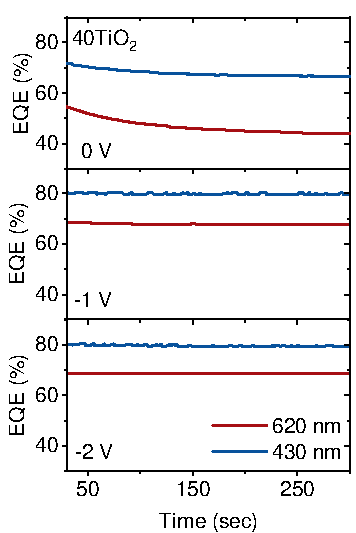
\includegraphics[width=\textwidth]{chapters/transport_layers/images/StaticEQE_40TiO2.pdf}
        \caption{}
        \label{}
    \end{subfigure}
    \hfill
    \begin{subfigure}{0.32\textwidth}
        \centering
        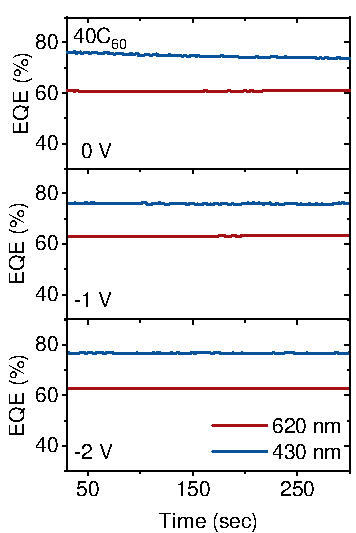
\includegraphics[width=\textwidth]{chapters/transport_layers/images/StaticEQE_40C60.pdf}
        \caption{}
        \label{}
    \end{subfigure}
    \hfill
    \begin{subfigure}{0.32\textwidth}
        \centering
        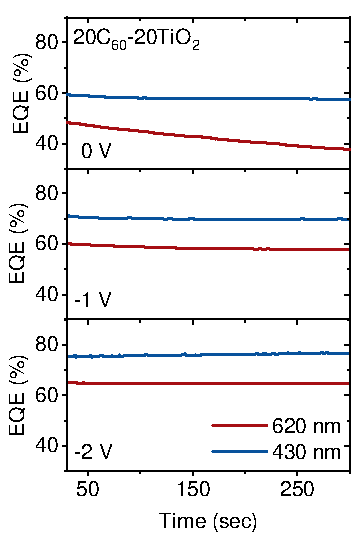
\includegraphics[width=\textwidth]{chapters/transport_layers/images/StaticEQE_20_20.pdf}
        \caption{}
        \label{}
    \end{subfigure}
    
    \caption[EQE as a function of time under steps of increasing reverse bias and two different illumination wavelengths (red - 620 nm and blue - 430 nm) for samples 40\ch{TiO_2}, 40\ch{C_{60}}, or 20\ch{C_{60}}-20\ch{TiO_2} as the ETL.]{EQE as a function of time under steps of increasing reverse bias and two different illumination wavelengths (red - 620 nm and blue - 430 nm) for samples (a) 40\ch{TiO_2}, (b) 40\ch{C_{60}}, and (c) 20\ch{C_{60}}-20\ch{TiO_2}. Between two consecutive measurements on the same PePD, an additional 300~s recovery period in dark was implemented.}
    \label{fig:etl_opt:static_eqe}
\end{figure}


Apart from the $J_d$ stability under the effect of reverse bias, evaluating the stability of the PePD's photo-response is as critical, considering that a common concern with perovskite-based solar cells is the loss of power conversion efficiency under continuous illumination \cite{Song2022CriticalAdditives, Fu2019I2Conditions,Khadka2021InsightsJunction}. To investigate this we monitored the EQE of samples 40\ch{TiO_{2}}, 40\ch{C_{60}}, and 20\ch{C_{60}}-20\ch{TiO_2} over time, applying consecutive reverse bias steps and using two different monochromatic illumination wavelengths (430 and 620 nm). Given that the samples are illuminated from the glass side, the absorption length of blue (430 nm) and red (620 nm) light are anticipated to correspond to the the HTL/perovskite and perovskite/ETL interface, respectively. Figure~\ref{fig:etl_opt:static_eqe} provides a summary of the results. At 0 V, samples 40\ch{TiO_2} and 20\ch{C_{60}}-20\ch{TiO_2} display an EQE decrease when illuminated with the 620 nm light source, which however is eliminated when increasing the reverse bias to -1 V. The EQE response at -2 V as a function of time is stable even for sample 40\ch{TiO_2}, which should already be undergoing a breakdown. This indicates that the breakdown current, which is generated and saturated by the recombination of electrons and holes that are injected form the HTL and ETL side, respectively, does not hinder the extraction of photo generated carriers. Besides, as revealed in Figure~\ref{fig:etl_opt:dynamicjv_eqe_staticjv}, the breakdown current is still two orders of magnitude lower compared to $J_{photo}$ at -2 V. Consequently, considering that the noise is dominated by shot noise originating from dark current, the device's specific detectivity (D*) will be mainly defined by the stability of $J_d$ under reverse bias, rather than the photoresponse. The calculation of shot-noise dominated D* relies on equation:  

\begin{equation}
    D^* = \frac{R}{\sqrt{2eJ_d}} \quad [Jones],
\end{equation}  

where R is the device's responsivity and e is the electron charge. In turn, the device's responsivity can be acquired from: 

\begin{equation}
    R = \frac{e}{hc/\lambda} \times EQE \quad [AW^{-1}],    
\end{equation}

where h is Planck's constant, c is the speed of light, and $\lambda$ is the incoming wavelength. Ignoring the thermal noise contributions is a common practice in thin-film photodetector research, however it admittedly leads to an overestimation of D* \cite{Martinez-Goyeneche2024Vacuum-DepositedDetection}. Nonetheless, this approximation allows for a qualitative comparison of the overall effects. For example, despite having similar EQE response under 620 nm illumination after 300 s at -2 V, sample 40\ch{TiO_2} would have one-order-of-magnitude lower D* compared to 20\ch{C_{60}}-20\ch{TiO_2} (equal to $8.8\times 10^{10}$ and  $8.8\times 10^{11}$ Jones, respectively). 

\begin{figure}[t]
    \centering
    % First row
    \begin{subfigure}[t]{0.4\textwidth}
        \centering
        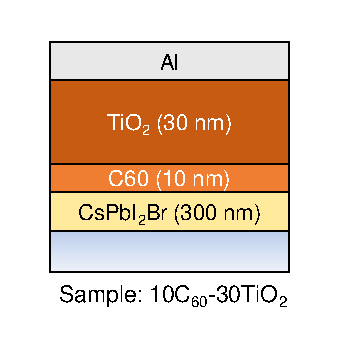
\includegraphics[width=\textwidth]{chapters/transport_layers/images/Sample_10_30_icon.pdf} % Replace with your image file
        \caption{}
        \label{}
    \end{subfigure}
    \hspace{0.5cm}
    \begin{subfigure}[t]{0.4\textwidth}
        \centering
        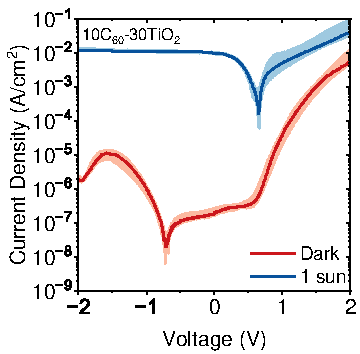
\includegraphics[width=\textwidth]{chapters/transport_layers/images/JV_Median_10_30.pdf} 
        % Replace with your image file
        \caption{}
        \label{}
    \end{subfigure} 
 % Second row
    \begin{subfigure}[t]{0.4\textwidth}
        \centering
        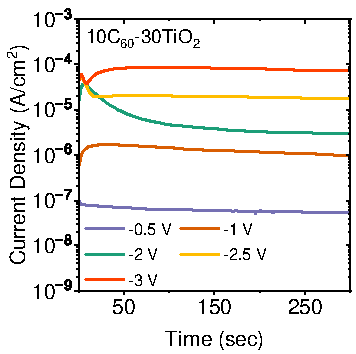
\includegraphics[width=\textwidth]{chapters/transport_layers/images/StaticJV_10_30.pdf} % Replace with your image file
        \caption{}
        \label{}
    \end{subfigure}
    \hspace{0.5cm}
    \begin{subfigure}[t]{0.4\textwidth}
        \centering
        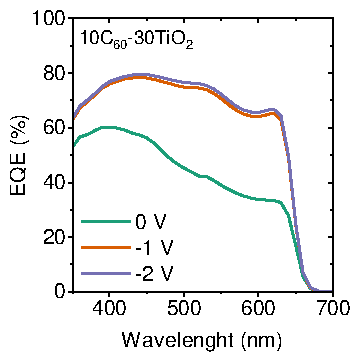
\includegraphics[width=\textwidth]{chapters/transport_layers/images/EQE_10_30.pdf} % Replace with your image file
        \caption{}
        \label{}
    \end{subfigure}
    \caption[Overview of electrical characterization results for PePDs with 10 nm of \ch{C_{60}} and 30 nm of \ch{TiO_2} as the ETL.]{Characterization of a PePD with 10 nm of \ch{C_{60}} and 30 nm of \ch{TiO_2} as the ETL. (a) Schematic illustration diode structure. (b) Current density as function of bias in dark and under 1-sun illumination. (c) Steady state measurement of current density as function of time in dark under steps of increasing reverse bias. (d) EQE as a function of wavelength under steps of increasing reverse bias.}
    \label{fig:etl_opt:10nmC60_30nmTiO2}
\end{figure}



With the results presented so far, it is clear that the deposition of 20 nm of \ch{C_{60}} between the perovskite and the \ch{TiO_2} layer is critical for the prevention of the PePD's breakdown under the effect of reverse bias. To determine whether a minimum \ch{C_{60}} thickness is required to ensure the device's reverse bias stability, we fabricated a fourth variation of the same stack, incorporating a 10 nm \ch{C_{60}} and a 30 nm \ch{TiO_2} layer as the ETL (sample 10\ch{C_{60}}-30\ch{TiO_2} in Figure~\ref{fig:etl_opt:10nmC60_30nmTiO2}a). The dynamic and static J-V scan, as well as the device's EQE are shown in Figure~\ref{fig:etl_opt:10nmC60_30nmTiO2}b-d, with the 3-order-of-magnitude increase of $J_d$ under the effect of -3 V revealing that 10 nm of \ch{C_{60}} are not in fact sufficient to fully protect the perovskite layer.




\subsection{Defect Analysis of the Perovskite/ETL Interface}


To further investigate the physical origin of the reverse bias instability of the 40\ch{TiO_2} sample as well as the performance variability the 40\ch{C_{60}}, we examine the EDS elemental concentration profiles of the three stacks, which are shown in Figure~\ref{fig:etl_opt:eds_concentration}a-c. Having as reference the onset of the \ch{Pb} signal, a dashed line is drawn in each plot to indicate the start of the perovskite layer. In contrast to sample 40\ch{C_{60}}, the Cs signal for sample 40\ch{TiO_2} is starting much earlier compared to Pb, I, and Br, pointing out to a significantly altered perovskite stoichiometry at the interface. The significant change in surface stoichiometry of the 40\ch{TiO_2} sample is likely responsible for increased inter-bandgap states, which enhance hole tunneling under reverse bias \cite{Huang2018IntrinsicCsPbI3, Kang2017HighCsPbBr3, Chu2020SoftDefects}. On the other hand, the elemental concentrations of sample 40\ch{C_{60}} reveal an overlapping of the Al signal and perovskite's constituents elements, further supporting the claim for incomplete surface coverage by the \ch{C_60} layer and the creation of metallic shorts that promote performance variability among devices fabricated on the same substrate. Finally, the elemental profile of sample 20\ch{C_{60}}-20\ch{TiO_2} indicates that the bilayer ETL configuration helps preserving the perovskite's surface stoichiometry, reducing the diffusion of Cs in the ETL (albeit not completely eliminating), while at the same time establishing a better separation between the Al contact and the perovskite. 



\begin{figure}[htbp]
    \centering
    \begin{subfigure}{0.32\textwidth}
        \centering
        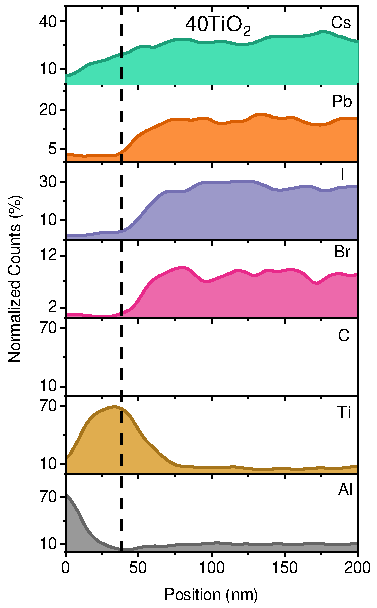
\includegraphics[width=\textwidth]{chapters/transport_layers/images/TEM_40TiO2.pdf}
        \caption{}
        \label{}
    \end{subfigure}
    \hfill
    \begin{subfigure}{0.32\textwidth}
        \centering
        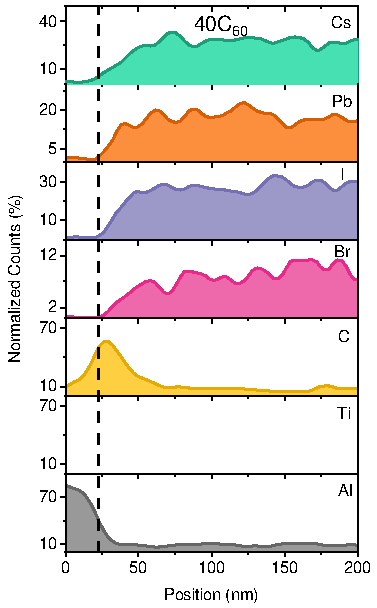
\includegraphics[width=\textwidth]{chapters/transport_layers/images/TEM_40C60.pdf}
        \caption{}
        \label{}
    \end{subfigure}
    \hfill
    \begin{subfigure}{0.32\textwidth}
        \centering
        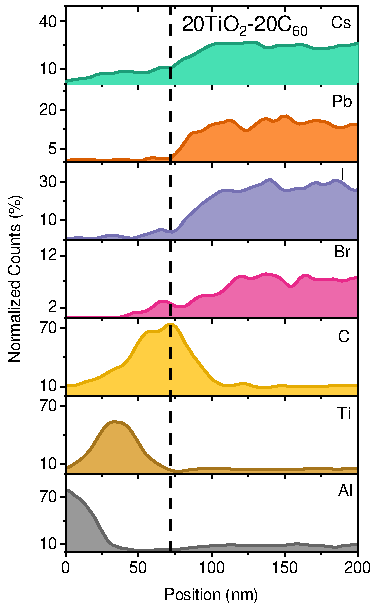
\includegraphics[width=\textwidth]{chapters/transport_layers/images/TEM_20_20.pdf}
        \caption{}
        \label{}
    \end{subfigure}
    
    \caption[EDS elemental concentration profiles for samples 40\ch{TiO_2}, 40\ch{C_{60}}, or 20\ch{C_{60}}-20\ch{TiO_2} as the ETL.]{EDS elemental concentration profiles for samples (a) 40\ch{TiO_2}, (b) 40\ch{C_{60}}, and (c) 20\ch{C_{60}}-20\ch{TiO_2}. Signal counts are normalized with respect to the total amount of counts at each depth position. The dashed line marks the beginning of the perovskite layer, based on the rise of the Pb signal.}
    \label{fig:etl_opt:eds_concentration}
\end{figure}

To further evaluate the perovskite/ETL interface quality we employ transient photocurrent (TPC) measurements, exciting the PePDs with two different light sources, a white and red (625 nm) light one. Their respective spectral profile is shown in Figure~\ref{fig:etl_opt:tpc_sources}a and b, where the LED irradiance has been tuned to yield a total intensity of 44.5 $mW/cm^2$ and 25.5 $mW/cm^2$ for the white and red light source, respectively. Using different light sources leads to different carrier generation profiles within the perovskite layer, enabling the disentanglement of bulk- and interface-dominated phenomena. The carrier generation rate as a function of distance inside the perovskite layer can be simulated using the optical constants of each device layer (obtained via spectroscopic ellipsometry) as an input in the transfer matrix algorithm (Figure~\ref{fig:tetl_opt:nk_transfer_materix})\cite{Burkhard2010AccountingCells}. The model developed for the simulation is illustrated in Figure~\ref{fig:etl_opt:tpc_simulation}a, while  the carrier generation rate within the \ch{CsPbI_2Br} layer for both light sources is shown in Figure~\ref{fig:etl_opt:tpc_simulation}b. 


\begin{figure}[ht!]
    \centering
    % First row
    \begin{subfigure}[t]{0.4\textwidth}
        \centering
        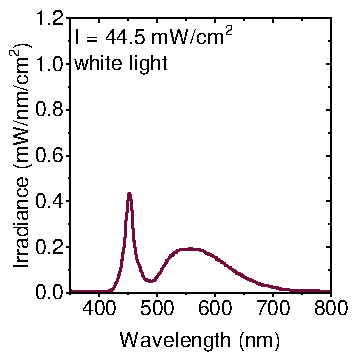
\includegraphics[width=\textwidth]{chapters/transport_layers/images/white_led.pdf} % Replace with your image file
        \caption{}
        \label{}
    \end{subfigure}
    \hspace{0.5cm}
    \begin{subfigure}[t]{0.4\textwidth}
        \centering
        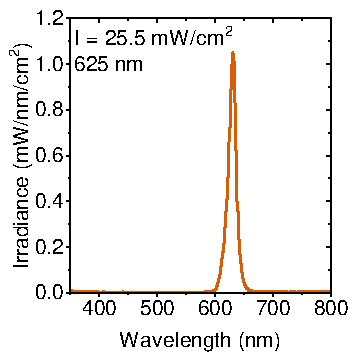
\includegraphics[width=\textwidth]{chapters/transport_layers/images/red_led.pdf} 
        % Replace with your image file
        \caption{}
        \label{}
    \end{subfigure} 

    \caption[Spectral power distribution of the white and red (625 nm) LED that were used for transient photocurrent measurements.]{Spectral power distribution of the (a) white and (b) red (625 nm) LED that were used for transient photocurrent measurements.}
    \label{fig:etl_opt:tpc_sources}
\end{figure}



\begin{figure}[htbp]
    \centering
    % Second row
    \begin{subfigure}[t]{0.99\textwidth}
        \centering
        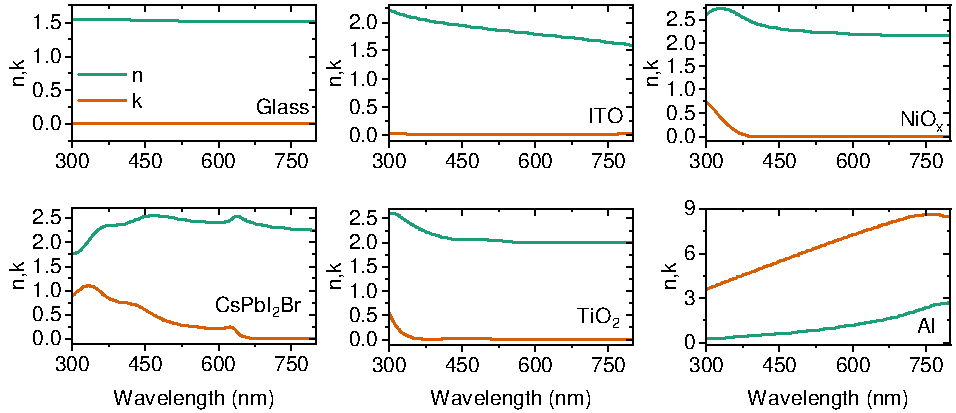
\includegraphics[width=\textwidth]{chapters/transport_layers/images/nk_transfer_matrix.pdf} % Replace with your image file
                
    \end{subfigure}
    \caption[Optical constants of all PePD layers used for the optical simulation of the 40\ch{TiO_2} sample.]{Optical constants of all PePD layers used for the optical simulation of the 40\ch{TiO_2} sample.}
    \label{fig:tetl_opt:nk_transfer_materix}
\end{figure}

\begin{figure}[ht!]
    \centering
     % Second row
    \begin{subfigure}[t]{0.4\textwidth}
        \centering
        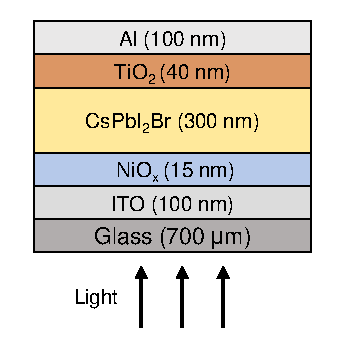
\includegraphics[width=\textwidth]{chapters/transport_layers/images/transfer_matrix_model.pdf} % Replace with your image file
        \caption{}
        \label{}
    \end{subfigure}
    \hspace{0.5cm}
    \begin{subfigure}[t]{0.4\textwidth}
        \centering
        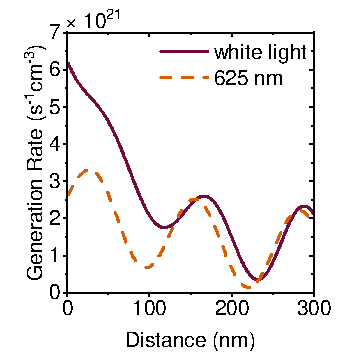
\includegraphics[width=\textwidth]{chapters/transport_layers/images/Generation_Rate.pdf} % Replace with your image file
        \caption{}
        \label{}
    \end{subfigure}
    \caption[Optical model for transfer-matrix algorithm simulations and simulated charge generation rate profiles.]{(a) Optical model used for the simulation of the charge generation rate across the perovskite layer based on the transfer-matrix algorithm. (b) Comparison of the charge generation rate across the perovskite thickness for illumination with the white and red light sources. The \ch{NiO_x}/\ch{CsPbI_2Br} interface corresponds to Distance = 0 nm, while the \ch{CsPbI_2Br}/\ch{TiO_2} interface corresponds to Distance = 300 nm.}
    \label{fig:etl_opt:tpc_simulation}
\end{figure}


A summary of the TPC results for all PePDs is provided in Figure~\ref{fig:etl_opt:tpc_comparison}a-d. For each sample and light source, the TPC response was measured at -1 and -2 V, with all curves normalized relative to the -2 V response. Starting with samples 40\ch{C_{60}} and 20\ch{C_{60}}-20\ch{TiO_2}, the photocurrent response under the effect of -1 and -2 V is similar for both illumination conditions. However, as the \ch{C_{60}} layer thickness decreases(samples 10\ch{C_{60}}-30\ch{TiO_2} and 40\ch{TiO_2}), a larger discrepancy under the effect of -1 and -2 V is observed. Specifically, the TPC response under -2 V has a square shape that corresponds to the light pulse that starts at 0 ms. In contrast, when the PePD is biased at -1 V, the photocurrent initially rises as a response to the light pulse but begins to decline within a few tens of microseconds, before starting to plateau at a lower value for the remainder of the light pulse. This effect is more pronounced under the effect of 625 nm illumination, although sample 40\ch{TiO_2} begins exhibiting this pattern even under white light illumination.


\begin{figure}[htbp]
    \centering
    \begin{subfigure}{0.24\textwidth}
        \centering
        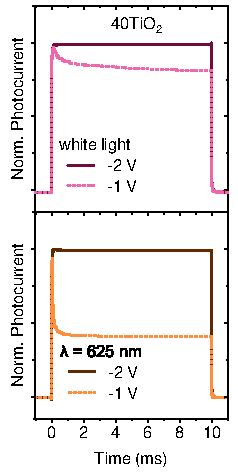
\includegraphics[width=\textwidth]{chapters/transport_layers/images/TPC_40TiO2.pdf}
        \caption{}
        \label{}
    \end{subfigure}
    \hfill
    \begin{subfigure}{0.24\textwidth}
        \centering
        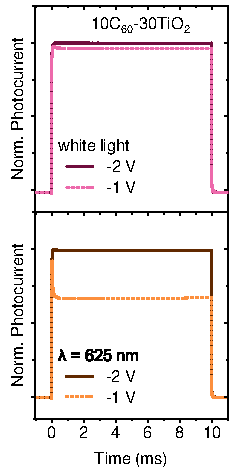
\includegraphics[width=\textwidth]{chapters/transport_layers/images/TPC_10_30.pdf}
        \caption{}
        \label{}
    \end{subfigure}
    \hfill
    \begin{subfigure}{0.24\textwidth}
        \centering
        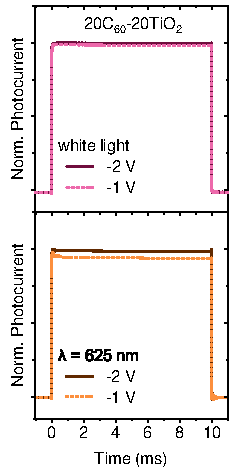
\includegraphics[width=\textwidth]{chapters/transport_layers/images/TPC_20_20.pdf}
        \caption{}
        \label{}
    \end{subfigure}
    \hfill
    \begin{subfigure}{0.24\textwidth}
        \centering
        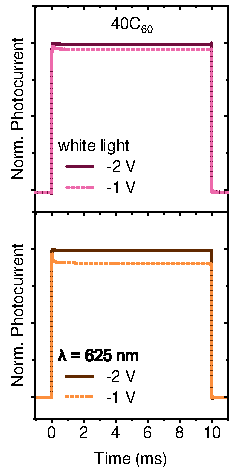
\includegraphics[width=\textwidth]{chapters/transport_layers/images/TPC_40C60.pdf}
        \caption{}
        \label{}
    \end{subfigure}
    
    \caption[Transient photocurrent response of samples 40\ch{TiO_2}, 10\ch{C_{60}}-30\ch{TiO_2}, 20\ch{C_{60}}-20\ch{TiO_2}, or 40\ch{C_{60}} as the ETL.]{Transient photocurrent response of samples (a) 40\ch{TiO_2}, (b) 10\ch{C_{60}}-30\ch{TiO_2}, (c) 20\ch{C_{60}}-20\ch{TiO_2}, and (d) 40\ch{C_{60}} when illuminated with a white (top) and red (bottom) light source, biased at -1 and -2 V. For each sample and illumination condition, the TPC response at -1 V has been normalized with respect to the TPC response at -2 V.}
    \label{fig:etl_opt:tpc_comparison}
\end{figure}

Such phenomena of transient peaks in the TPC response of organic- and perovskite-based photodiodes were previously associated with a non-ideal charge extraction and carrier accumulation at an interface \cite{Neophytou2019EnhancingLayer, Hwang2009Drift-diffusionCells,Mcneill2009PhotocurrentEffects}. Specifically, in the presence of a defect-rich interface, in this case the perovskite/ETL interface, electrons may get trapped near the anode, leading to a local reduction of the electric field via the creation of a space-charge region. This in turn limits charge separation and promotes recombination \cite{Mcneill2009PhotocurrentEffects}. The electron trapping rate, and by extension the width of the space charge region, depends of course on the interface's defect density but also the charge generation rate in the same region \cite{Hwang2009Drift-diffusionCells}. However, Figure~\ref{fig:etl_opt:tpc_simulation}b revealed that the charge generation rate at the perovskite/ETL interface (Distance = 300 nm) is similar for both white and red light illumination, and equal to approximately $2\times 10^{21}s^{-1}cm^{-3}$. As a result, and taking as example the 40\ch{TiO_2} sample, we could reasonable consider similar levels of trapped-charge accumulation at the perovskite/ETL interface for both types of illumination, leading to the formation of a space-charge region of similar width. Yet, as shown in Figure~\ref{fig:etl_opt:tpc_comparison}a, the transient peak is more pronounced under the effect of red light illumination. This is attributed to the fact that under white light illumination a larger percentage of carriers is generated closer to HTL/perovskite interface (Distance = 0 nm in Figure~\ref{fig:etl_opt:tpc_simulation}b), which can be more efficiently separated and extracted, dominating in the sample's TPC response. In conclusion, the diminishing TPC peak under red light illumination and -1 V bias with increasing \ch{C_{60}} layer thickness is further supporting the claim that the reverse bias breakdown is eliminated through a reduction in the density of interface trap states.

Interestingly, the saturated TPC response of sample 40\ch{TiO_2} under 625 nm light illumination at -1 V is almost half compared to -2 V. On the other hand, the saturated EQE response of the same sample at 620 nm (Figure~\ref{fig:etl_opt:static_eqe}a) is approximately equal to 70\% when the PePD is biased at -1 and -2 V. This discrepancy is attributed to the significantly lower intensity of the EQE light source (<3 $mW/cm^2$) when compared to the red light source of the TPC setup (25.5 $mW/cm^2$) and the fact that the accumulation of trapped charge at the perovskite/ETL interface is directly proportional to it \cite{Hwang2009Drift-diffusionCells,Mcneill2009PhotocurrentEffects}.

\subsection{Enhancement of Response Speed}

\begin{figure}[ht!]
    \centering
    % First row
    \begin{subfigure}[t]{0.4\textwidth}
        \centering
        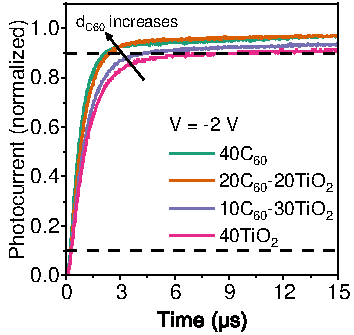
\includegraphics[width=\textwidth]{chapters/transport_layers/images/TPC_comparison_v2.pdf} % Replace with your image file
        \caption{}
        \label{}
    \end{subfigure}
    \hspace{0.5cm}
    \begin{subfigure}[t]{0.37\textwidth}
        \centering
        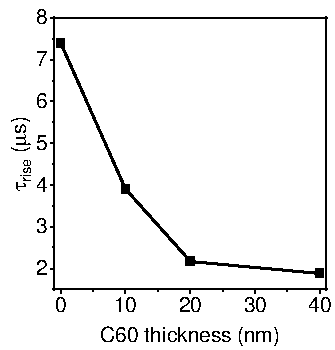
\includegraphics[width=\textwidth]{chapters/transport_layers/images/Rise_time_f_c60_thickness.pdf} 
        % Replace with your image file
        \caption{}
        \label{}
    \end{subfigure} 
 
    \caption[Comparison of the TPC response time of PePDs with various combinations of the \ch{C_{60}}-\ch{TiO_2} bi-layer configuration and dependence of the PePD's rise time ($\tau_r$) on the thickness of the \ch{C_{60}} layer.]{(a) Comparison of the TPC response time of PePDs with various combinations of the \ch{C_{60}}-\ch{TiO_2} bi-layer configuration when illuminated by the white light source and biased at -2 V. (b) Dependence of the PePD's rise time ($\tau_r$) on the thickness of the \ch{C_{60}} layer deposited on top of the perovskite layer.}
    \label{fig:etl_opt:rise_time}
\end{figure}

Besides the investigation of the perovskite/ETL interface quality, the TPC measurements can be further used to evaluate the carrier extraction speed of the PePDs, which is defined as the time it takes for the device to respond to the transient light pulse. Figure~\ref{fig:etl_opt:rise_time}a superimposes the photoresponse of the four PePDs, biased at -2 V, during the first microseconds of the measurement under white light illumination. A distinct trend emerges, where the response becomes faster as the \ch{C_{60}} layer thickness increases. The PePDs' rise time ($\tau_r$) can be further quantified as the time required for the photocurrent to reach 90\% of its steady-state value (starting from 10\%). Figure~\ref{fig:etl_opt:rise_time}b displays the extracted $\tau_r$ as a function of the \ch{C_{60}} layer thickness, highlighting the impact of the chosen ETL configuration on the detector's speed.  

\begin{figure}[htbp]
    \centering
    \begin{subfigure}{0.32\textwidth}
        \centering
        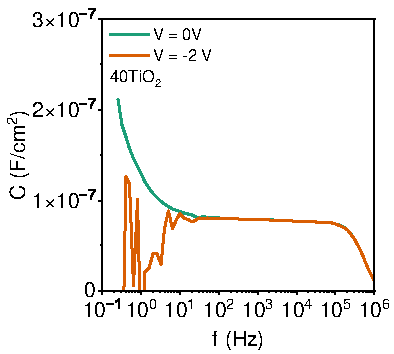
\includegraphics[width=\textwidth]{chapters/transport_layers/images/Cf_40TiO2.pdf}
        \caption{}
        \label{}
    \end{subfigure}
    \hfill
    \begin{subfigure}{0.32\textwidth}
        \centering
        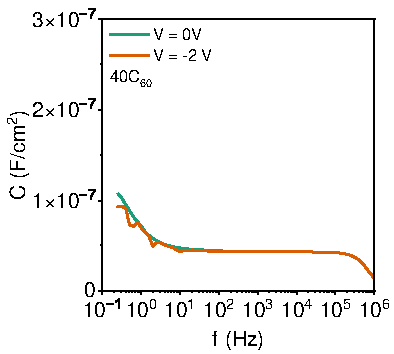
\includegraphics[width=\textwidth]{chapters/transport_layers/images/Cf_40C60.pdf}
        \caption{}
        \label{}
    \end{subfigure}
    \hfill
    \begin{subfigure}{0.32\textwidth}
        \centering
        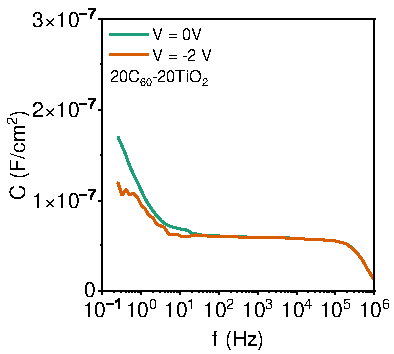
\includegraphics[width=\textwidth]{chapters/transport_layers/images/Cf_20_20.pdf}
        \caption{}
        \label{}
    \end{subfigure}
    
    \caption[Frequency-dependent capacitance for samples with various combinations of the \ch{C_{60}}-\ch{TiO_2} bi-layer configuration.]{Frequency-dependent capacitance for samples (a) 40\ch{TiO_2}, (b) 40\ch{C_{60}}, and (c) 20\ch{C_{60}}-20\ch{TiO_2}, biased at 0 V and -2 V. The collapse of the capacitance for sample 40\ch{TiO_2} at -2 V and frequencies below 10 Hz is another aftermath of the breakdown mechanism that is triggered under the effect of prolonged reverse bias.}
    \label{fig:etl_opt:cf_all}
\end{figure}

\begin{figure}[ht!]
    \centering
    
 % Second row
    \begin{subfigure}[t]{0.45\textwidth}
        \centering
        %\hspace{-1.5cm}
        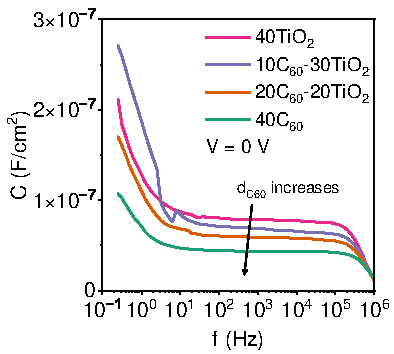
\includegraphics[width=\textwidth]{chapters/transport_layers/images/Cf_comparison.pdf} % Replace with your image file
        
    \end{subfigure}
    \caption[Comparison of the frequency-dependent capacitance of PePDs with various combinations of the \ch{C_{60}}-\ch{TiO_2} bi-layer configuration.]{Comparison of the frequency-dependent capacitance of PePDs with various combinations of the \ch{C_{60}}-\ch{TiO_2} bi-layer configuration, without the application of any external bias. }
    \label{fig:etl_opt:capacitance}
\end{figure}


Considering that the RC time constant is critical for a photodiode's response speed, we characterize the devices' capacitance as a function of frequency at 0 and -2 V (Figure~\ref{fig:etl_opt:cf_all}a-c). For frequencies above 10 Hz, samples 40\ch{C_{60}} and 20\ch{C_{60}}-20\ch{TiO_2} have identical capacitance at 0 and -2 V, revealing that the built-in potential is sufficient to fully deplete the PePDs, without the need for additional reverse bias. This further suggests that the increase in the devices' response speed when a thicker \ch{C_{60}} layer is used can not be attributed to an extension of the depletion region within the perovskite layer itself \cite{Goushcha2017OnPhotodiodes}. The signal of the capacitance measurement for sample 40\ch{TiO_2} exhibits the same trend, even though at -2 V operation it is collapsing to 0 and becomes more noisy for frequencies below 10 Hz, a direct aftermath of the device breakdown after reverse biasing for prolonged duration. Figure~\ref{fig:etl_opt:capacitance} provides an overlay comparison of the C-f measurement for all PePDs in absence of any external bias. For moderate frequencies, in the range of 10Hz to 100 kHz, the capacitance of the device is inversely proportional to the thickness of the \ch{C_{60}} layer, in agreement with the observed increase in response speed ($\tau_r \propto \tau_{RC}$). Considering that the equivalent device capacitance for a series connection is equal to 
 
 \begin{equation}
    \frac{1}{C_{eq}} = \frac{1}{C_{pvkt}} + \frac{1}{C_{ETL}},
    \label{eg:series_cap}
 \end{equation}

 the decrease in $C_{eq}$ could potentially be attributed to an extension of the depletion width within the \ch{C_{60}} layer, as it was previously numerically shown and attributed to the relatively low doping density of the material \cite{Pham2023EffectsCells}.  

\begin{table}[htbp]
    \centering
    \caption{Parameters used for the estimation of the perovskite’s $\epsilon_r$ according to the capacitance measurements of the 40\ch{TiO_2} sample. }
    \renewcommand{\arraystretch}{1.5}
    \begin{tabular}{| c | c | c | c |}
        \hline
        C [$F/cm^2$] & $\epsilon_0$ [$F/m$] & $d_{pvkt}$ [$nm$] & A [$cm^2$] \\
        \hline
        $7.8\times10^{-8}$ & $8.85\times10^{-12}$ & 300 & 0.125 \\
        \hline
    \end{tabular}
    
    \label{tab:etl_opt:er_from_pepd}
\end{table}

\begin{figure}[htbp]
    \centering
    % First plot
    \begin{subfigure}[t]{0.4\textwidth} % Adjust width as needed
        \centering
        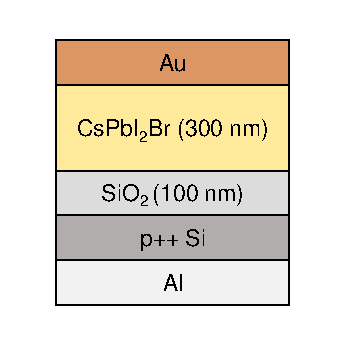
\includegraphics[width=\textwidth]{chapters/transport_layers/images/MOS_Structure_icon.pdf} % Replace with your image
        \caption{}
        \label{}
    \end{subfigure}
    \hspace{0.5cm}
    % Second plot
    \begin{subfigure}[t]{0.4\textwidth} % Adjust width as needed
        \centering
        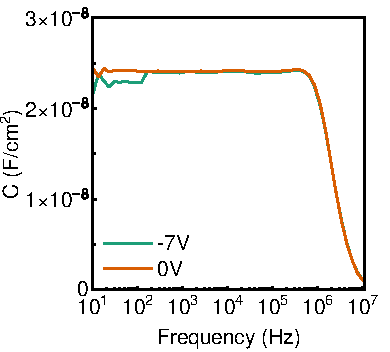
\includegraphics[width=\textwidth]{chapters/transport_layers/images/MOS_IS.pdf} % Replace with your image
        \caption{}
        \label{}
    \end{subfigure}

    % Caption for the whole figure
    \caption[Schematic illustration of perovskite MOS capacitor and frequency-dependent capacitance results.]{(a) Schematic illustration of the MOS capacitor, fabricated for the evaluation of the perovskite's relative permittivity. (b) Frequency dependent capacitance of the MOS structure under the effect of 0 V and -7 V. }
    \label{etl:mos_stack}
\end{figure}


\begin{table}[htbp]
    \centering
    \caption{Parameters used for the estimation of the perovskite’s $\epsilon_r$ according to the capacitance measurements of the MOS structure.}
    \renewcommand{\arraystretch}{1.5}
    \begin{tabular}{| c | c | c | c | c | c |}
        \hline
        $C_{eq}$ [$F/cm^2$] & $\epsilon_0$ [$F/m$] & $\epsilon_{r,SiO_2}$ & $d_{SiO_2}$ [$nm$] & $d_{pvkt}$ [$nm$] & A [$cm^2$] \\
        \hline
        $2.4\times10^{-8}$ & $8.85\times10^{-12}$ & 3.9 & 100 & 300 & 0.16 \\
        \hline
    \end{tabular}
    
    \label{tab:etl_opt:er_from_mos}
\end{table}



To verify this hypothesis, we first extract perovskite's relative permittivity ($\epsilon_r$) from the C-f of sample 40\ch{TiO_2}, considering that the depletion region is limited within the \ch{CsPbI_2Br} layer and using equation $C_{pvkt} = \frac{\epsilon_r\epsilon_0A}{d}$, where $\epsilon_0$ is the vacuum permittivity, $A$ is the device area and $d$ is the perovskite thickness. Using the values that are summarized in Table~\ref{tab:etl_opt:er_from_pepd}, we extract $\epsilon_r = 26.5$. In order to corroborate this value and eliminate the influence of the ETL, we additionally fabricate a metal-oxide-semiconductor (MOS) capacitor, that employs heavily a p-doped silicon wafer as the metal contact and a thermally-grown \ch{SiO_2} (100 nm) layer as the oxide. The schematic of the MOS-stack, as well as the results of the C-f measurement at 0 and -7 V are shown in Figure~\ref{etl:mos_stack}a and b, respectively. Taken into account that the perovskite and oxide are connected in series (eq.~\ref{eg:series_cap}) and using the values of Table~\ref{tab:etl_opt:er_from_mos}, we extract $\epsilon_r = 26.9$, which is in great agreement with the value that was estimated from the 40\ch{TiO_2} sample. Finally, Figure~\ref{fig:etl_opt:capacitance_numerical_measured} compares the measured and numerically calculated equivalent capacitance of the PePDs as function of the \ch{C_{60}} layer, considering that the latter is fully depleted. The strong agreement between measured and calculated values further confirms our initial hypothesis that the increase in the PePDs response speed with increasing \ch{C_{60}} layer thickness is attributed to a reduction of the stack's RC constant, though an extension of the depletion area towards the \ch{C_{60}} layer \cite{Goushcha2017OnPhotodiodes}. 


\begin{figure}[ht!]
    \centering
    
    \begin{subfigure}[t]{0.45\textwidth}
        \centering
        \includegraphics[width=\textwidth]{chapters/transport_layers/images/C_f_c60_thick.pdf} % Replace with your image file
    \end{subfigure}
    \caption[Comparison of the experimentally extracted PePD capacitance with the analytically calculated values.]{Comparison of the experimentally extracted PePD capacitance at $10^3$ Hz with the analytically calculated value, considering the extension of the depletion region into the \ch{C_{60}} layer.}
    \label{fig:etl_opt:capacitance_numerical_measured}
\end{figure}



\begin{figure}[htbp]
    \centering
    \begin{subfigure}{0.32\textwidth}
        \centering
        \includegraphics[width=\textwidth]{chapters/transport_layers/images/JV_40C60_20TiO2.pdf}
        \caption{}
        \label{}
    \end{subfigure}
    \hfill
    \begin{subfigure}{0.32\textwidth}
        \centering
        \includegraphics[width=\textwidth]{chapters/transport_layers/images/EQE_40C60_20TiO2.pdf}
        \caption{}
        \label{}
    \end{subfigure}
    \hfill
    \begin{subfigure}{0.3\textwidth}
        \centering
        \includegraphics[width=\textwidth]{chapters/transport_layers/images/40C60-20TiO2-rise.pdf}
        \caption{}
    \end{subfigure}
    
    \caption[Overview of electrical characterization for a PePD that features a 40 nm \ch{C_{60}} and a 20 nm \ch{TiO_2} bi-layer as the ETL.]{Characterization of PePD that features a 40 nm \ch{C_{60}} and a 20 nm \ch{TiO_2} bi-layer as the ETL. (a) Current density as a function of bias in dark and under 1-sun illumination. (b) EQE as a function of wavelength under steps of increasing reverse bias. (c) TPC response time for while light illumination and -2 V bias.}
    \label{fig:etl_opt:40C60_20TiO2}
\end{figure}



This finding implies that the carrier extraction speed could be improved by further increasing the thickness of the \ch{C_{60}} layer. To evaluate this hypothesis, we fabricated an additional sample whose ETL comprised of 40 nm of \ch{C_{60}} and 20 nm of \ch{TiO_2} (sample 40\ch{C_{60}}-20\ch{TiO_2}). The dynamic J-V scan, the spectral EQE, as well as the transient photocurrent of the respective PePD are shown in Figure~\ref{fig:etl_opt:40C60_20TiO2}a-c. Indeed, for a device of 0.125 $cm^2$ area, an almost 10\% decrease of $\tau_r$ is achieved (from 2.17 to 1.96 $\mu s$) with regards to the 20\ch{C_{60}}-20\ch{TiO_2} sample. However, when examining the EQE spectra of the 40\ch{C_{60}}-20\ch{TiO_2} sample, it is observed that the EQE does no longer saturate at -1 V, while remaining below 70\% even when increasing the reverse bias up to -2 V. This is in stark contrast to what was observed for sample the 20\ch{C_{60}}-20\ch{TiO_2} sample (Figure~\ref{fig:etl_opt:dynamicjv_eqe_staticjv}f), whose EQE response was already saturated and beyond 70\% at -1 V. Nevertheless, this trend is consistent with previous literature reports that showcased a decrease of a perovskite-based solar cell's PCE when the \ch{C_{60}} layer thickness was increased beyond 20 nm \cite{Klipfel2022C60Layer}.


\begin{figure}[htbp]
    \centering
    \begin{subfigure}{0.35\textwidth}
        \centering
        \includegraphics[width=\textwidth]{chapters/transport_layers/images/Capacitance_f_area.pdf}
        \caption{}
        \label{}
    \end{subfigure}
    \hfill
    \begin{subfigure}{0.3\textwidth}
        \centering
        \includegraphics[width=\textwidth]{chapters/transport_layers/images/TPC_f_area.pdf}
        \caption{}
        \label{}
    \end{subfigure}
    \hfill
    \begin{subfigure}{0.29\textwidth}
        \centering
        \includegraphics[width=\textwidth]{chapters/transport_layers/images/Rise_time_farea.pdf}
        \caption{}
        \label{}
    \end{subfigure}
    
    \caption[Impact of PePD contact size on the electrical characteristics of the 40\ch{C_{60}} sample.]{Impact of PePD contact size on the characteristics of the 40\ch{C_{60}} sample. (a) Frequency-dependent capacitance at 0 V, (b) TPC response time under white light illumination and -2 V bias, and (c) dependence of PePD's rise time on device area.}
    \label{fig:etl_opt:dev_area}
\end{figure}

As a result, depending on the application, a trade-off between speed and charge carrier extraction efficiency may be necessary. However, this trade-off can avoided by reducing the diode's area, which in turn decreases its capacitance and enhances $\tau_r$ without compromising the EQE. To demonstrate this, we reduced the contact area of sample 40\ch{C_{60}} from 0.125 $cm^2$ to 0.075 $cm^2$ and 0.025 $cm^2$. Figure~\ref{fig:etl_opt:dev_area}a illustrates the resulting decrease in capacitance, while Figure~\ref{fig:etl_opt:dev_area}b shows the corresponding increase in response speed. The extracted $\tau_r$ as function of area, shown in Figure~\ref{fig:etl_opt:dev_area}c, exhibits a linear relationship. For the device with 0.025 $cm^2$ area, $\tau_r$ approaches 1 $\mu s$, which approaches the detection limit of the setup, yet sub-$\mu s$ response speeds can be projected with further pixel miniaturization.

To benchmark the performance of our PePDs against prior studies utilizing thermally evaporated inorganic perovskites (\ch{CsPbI_2Br}, with X = I, Br, Cl, or their combinations) in photodiode fabrication, we provide a comparative summary of key device parameters in Table~\ref{tab:device_summary}. Among the available literature, only the study by Yang et al. evaluates PePD behavior under a -2 V bias, a condition under which their device operates in photoconductive gain mode (EQE > 100\%), leading to unusually high responsivity and specific detectivity \cite{Yang2019High-QualityApplications}. Other reported devices either function in "self-powered" mode (0 V bias) or operate under a modest reverse bias of -0.5 V. In contrast, our work distinctly demonstrates stable and efficient operation at -2 V, delivering the lowest $J_d$ in this bias range and a competitive response time, all without compromising the aspect of responsivity.


\clearpage
\begin{sidewaystable}[H]
\centering
\caption{Summary of the characteristic parameters of photodiodes with a thermally evaporated (co-evaporation, sequential evaporation, single source evaporation) \ch{CsPbX_3} active layer, where X represents I, Br, Cl, or their combinations.}
\small
\renewcommand{\arraystretch}{1.5}
\begin{tabular}{|
  >{\centering\arraybackslash}p{4cm} |
  >{\centering\arraybackslash}p{0.8cm} |
  >{\centering\arraybackslash}p{2cm} |
  >{\centering\arraybackslash}p{0.8cm} |
  >{\centering\arraybackslash}p{1.1cm} |
  >{\centering\arraybackslash}p{2.1cm} |
  >{\centering\arraybackslash}p{1.4cm} |
  >{\centering\arraybackslash}p{0.9cm} |
  >{\centering\arraybackslash}p{0.8cm} |
}
\hline
\makecell{\textbf{Device}} &
\makecell{\textbf{Bias} \\ \textbf{[V]}} &
\makecell{\textbf{J\textsubscript{d}} \\ \textbf{[A/cm\textsuperscript{2}]}} &
\makecell{$\lambda$ \\ \textbf{[nm]}} &
\makecell{\textbf{R} \\ \textbf{[A/W]}} &
\makecell{\textbf{D\textsuperscript{*}} \\ \textbf{[Jones]}} &
\makecell{\textbf{$\tau$\textsubscript{r}/$\tau$\textsubscript{f}} \\ \textbf{[$\mu$s]}} &
\makecell{\textbf{Area} \\ \textbf{[cm\textsuperscript{2}]}} &
\makecell{\textbf{Ref.}} \\
\hline
\makecell{ITO/Ca/C60/CsPbCl3/\\TAPC/TAPC:MoOx\\/MoOx/Ag} 
 & -2 & $\sim7\times 10^{-6}$ & 365 & 2.27 & $1.4\times 10^{13}\dagger$ & 46/46 & - & \cite{Yang2019High-QualityApplications} \\
\hline
\makecell{ITO/CuPC/CsPbBr3\\/MoO3/Ag}
& 0 & $\sim2.2\times 10^{-8}$ & 500 & 0.31 & $5.22\times 10^{12}$\# & 0.96/4.4 & 0.09 & \cite{Liu2020EnhancingSensing} \\
\hline
\multirow{2}{*}{\makecell{ITO/NiO/CsPbI3/TiO2/Al}} 
  & -0.5 & $1\times10^{-7}$ & 530 & 0.34 & $2\times10^{12}$\# & 7/8 & \multirow{2}{*}{0.025} & \multirow{2}{*}{\cite{PintorMonroy2021All-EvaporatedApplications}} \\
\cline{2-7}
  & -2 & $\sim1-4\times10^{-6}$ & - & - & - & - &  & \\
\hline
\multirow{2}{*}{\makecell{FTO/cp-TiO2/mp-TiO2/\\CsPbCl3/Spiro-PT/Au}} 
  & 0 & $9.7\times10^{-10}$ & 406 & 0.118 & $6.62\times10^{12}$\# & 0.12/0.82 & \multirow{2}{*}{0.1} & \multirow{2}{*}{\cite{Ji2022UltrafastDeposition}} \\
\cline{2-7}
  & -1.5 & $\sim1\times10^{-6}$ & - & - & - & - & & \\
\hline
\multirow{2}{*}{\makecell{ITO/NiOx/CsPbI2Br/\\C60/TiO2/Al}} 
  & \multirow{2}{*}{\makecell{-2}}  & $*4.5\times10^{-7}$ & \multirow{2}{*}{\makecell{620}} & \multirow{2}{*}{\makecell{0.33}} & $8.8\times10^{11}$\# & \multirow{2}{*}{\makecell{2.17/1.92}} & \multirow{2}{*}{0.125} & \multirow{2}{*}
  {\makecell{This\\work}} \\
\cline{3-3} \cline{6-6}
  &  & $1\times10^{-6}$ &  &  & $5.9\times10^{11}$\# & & & \\
\hline
\end{tabular}
\vspace{1.5em} % small vertical space
\begin{minipage}{0.95\textwidth}
\small
\begin{itemize}
    \item[$\dagger$] D* derived from spectral density.
    \item[\#] D* calculated from $J_d$ assuming that the shot noise is the dominant one.
    \item[*] $J_d$ values derived from steady-state scans. The rest are extracted from dynamic J-V scans.
    \item[$\sim$] $J_d$ values approximated from the provided plots or relevant information, without being explicitly defined in the text.
\end{itemize}
\end{minipage}
\label{tab:device_summary}
\end{sidewaystable}
\clearpage

\section{Development of Top-Illuminated PePDs}

\begin{figure}[ht!]
    \centering
    
     \raisebox{0.1cm}{ % Move this figure up by 1.5 cm (adjust as needed)
    \begin{subfigure}{0.3\textwidth}
        \centering
        \includegraphics[width=\textwidth]{chapters/transport_layers/images/pix_stack_cross_section.pdf}
        \vspace{4mm}
        \caption{}
        \label{}
    \end{subfigure}
    }
    \hspace{0.5cm}
    \begin{subfigure}{0.4\textwidth}
        \centering
        \includegraphics[width=\textwidth]{chapters/transport_layers/images/AP40_4_JV.pdf}
        \caption{}
        \label{}
    \end{subfigure}
    
    \vspace{0.5em} % Optional vertical spacing between rows
    
    \begin{subfigure}{0.4\textwidth}
        \centering
        \includegraphics[width=\textwidth]{chapters/transport_layers/images/AP40_4_EQE.pdf}
        \caption{}
        \label{}
    \end{subfigure}
    \hspace{0.5cm}
    \begin{subfigure}{0.4\textwidth}
        \centering
        \includegraphics[width=\textwidth]{chapters/transport_layers/images/AP40_4_EQE_fV.pdf}
        \caption{}
        \label{}
    \end{subfigure}
    
    \caption[Overview of electrical characterization for a top-illuminated PePD that features 20 nm of \ch{C_{60}} and 20 nm of \ch{TiO_2} as the ETL.]{Characterization of a top-illuminated PePD with 20 nm of \ch{C_{60}} and 20 nm of \ch{TiO_2} as the ETL. (a) Schematic illustration of diode structure. (b) Current density as a function of bias in dark and under 1-sun illumination. (c) EQE as a function of wavelength under steps of increasing reverse bias. (d) EQE as a function of bias under monochromatic 500 nm illumination.}
    \label{fig:pix_pepd:cross_section_performance}
\end{figure}

Benefiting from the reliable and competitive performance of the bottom-illuminated photodiodes, we proceed to the fabrication and characterization of top-illuminated photodiodes, whose cross-section is illustrated in Figure~\ref{fig:pix_pepd:cross_section_performance}a. The optimal ETL configuration of 20 nm of \ch{C_{60}} and 20 nm of \ch{TiO_2} is selected for the top-illuminated PePDs, as well. For this type of photodetectors, $J_d$ at -2 V is maintained below 4 $\mu A/cm^2$, while $J_{photo}$ surpasses 10 $mA/cm^2$ in the same biasing point (Figure~\ref{fig:pix_pepd:cross_section_performance}b). Additionally, the EQE response is close to 60\% and mostly saturated at -1 V (Figure~\ref{fig:pix_pepd:cross_section_performance}c). The main difference compared to the performance of respective the bottom-illuminated PePDs (Figure~\ref{fig:etl_opt:dynamicjv_eqe_staticjv}c) is the delayed saturation of $J_{photo}$ and EQE as a function of reverse bias. This "turning-on" delay is more clearly illustrated in Figure~\ref{fig:pix_pepd:cross_section_performance}d, which demonstrates the EQE as a function of bias under constant mono-chromatic illumination of 500 nm, and indicates the presence of an energetic barrier that must be overcome to allow the efficient extraction of the photo-generated carriers. 

\begin{figure}[htbp]
    \centering
    % First row
    \begin{subfigure}[t]{0.49\textwidth}
        \centering
        \includegraphics[width=\textwidth]{chapters/material_properties/images/TEM_As_Dep.pdf} % Replace with your image file
        \caption*{(a)}
    \end{subfigure}
    \hfill
    \begin{subfigure}[t]{0.49\textwidth}
        \centering
        \includegraphics[width=\textwidth]{chapters/material_properties/images/TEM_5_min.pdf} % Replace with your image file
        \caption*{(b)}
    \end{subfigure}

    \vspace{0.5cm}
    % Second row
    \begin{subfigure}[t]{0.35\textwidth}
        \centering
        \includegraphics[width=\textwidth]{chapters/transport_layers/images/TiN-NiO Interface_As_Dep.pdf} % Replace with your image file
        \caption*{(c)}
    \end{subfigure}
    \hspace{1.2cm}
    \begin{subfigure}[t]{0.35\textwidth}
        \centering
        \includegraphics[width=\textwidth]{chapters/transport_layers/images/TiN-NiO Interface_5min.pdf} % Replace with your image file
        \caption*{(d)}
    \end{subfigure}
    \caption[EDS elemental concentration and ABF-STEM of an as-deposited and an annealed Si/TiN substrate.]{EDS elemental concentration of a Si/TiN substrate with a \ch{NiO_x} layer that is (a) as-deposited and (b) annealed for 5 minutes at 300 \degree C in open air. ABF-STEM of the respective (c) as-deposited and (d) annealed Si/TiN/\ch{NiO_x} samples.}
    \label{fig:pix_pepd:tem_on_nio}
\end{figure}

Considering that such barrier was not present during the development of the stack on top of the glass/ITO substrates, we turn to the Si/TiN substrate and its interface with the DC-sputtered \ch{NiO_x} layer. Two \ch{NiO_x}-coated Si/TiN substrates were examined using transmission electron microscopy (TEM) on a focused ion beam (FIB)-prepared cross-section. The first substrate features the \ch{NiO_x} layer in its as-deposited state (Figure\ref{fig:pix_pepd:tem_on_nio}a and c), while the second one underwent a 5-minute annealing at 300\degree C in ambient conditions, replicating the step used in device fabrication (Figure\ref{fig:pix_pepd:tem_on_nio}b and d). Figure~\ref{fig:pix_pepd:tem_on_nio}b clearly illustrates the effect of annealing on the \ch{NiO_x} layer, marked by the elimination of the gap between the atomic concentrations of Ni and O in the relevant region. For both the as-deposited and 5-min annealed film, a thin \ch{TiO_x} layer is formed between the TiN contact and the \ch{NiO_x} transport layer. The thickness of the oxide layer appears to be unaffected by the annealing step, suggesting that the oxidation is either native to the TiN contacts or  occurs during the \ch{NiO_x} deposition itself—potentially exacerbated by the plasma environment within the vacuum chamber. As a result, the formation of this thin \ch{TiO_x} layer could be held accountable for the presence of the energy barrier in the top-illuminated PePDs. 

This issue could be possible resolved with the replacement of TiN with a non-oxidizing contact. During the time of this study, the only fab-compatible alternative was the use of copper as the bottom contact. However, Cu is known to severely oxidize under elevated temperatures, rendering it an unsuitable choice for our thermally-stable PePDs. As a result, future efforts on the elimination of the \ch{TiO_x} barrier should be focused on the choice and processing conditions of the HTL, the introduction of passivation layers that prevent oxidation or the inversion of the stack. 

\begin{figure}[htbp]
    \centering
    % First row
    \begin{subfigure}[t]{0.46\textwidth}
        \centering
        \includegraphics[width=\textwidth]{chapters/transport_layers/images/AP38_9_Static.pdf} % Replace with your image file
      
    \end{subfigure}
    \hfill
    \begin{subfigure}[t]{0.44\textwidth}
        \centering
        \includegraphics[width=\textwidth]{chapters/transport_layers/images/Responsivity_Detectivity.pdf} % Replace with your image file
       
    \end{subfigure}

    \caption[Steady-state current density, responsivity, and specific detectivity of top-illuminated PePD.]{(a) Steady-state measurement of current density as a function of time in dark under steps of increasing reverse bias for the top-illuminated PePD. (b) Responsivity and (c) specific detectivity of the top illuminated PePD as a function of wavelength, measured at -1 and -2 V. }
    \label{fig:etl:top_illuminated_stability_detectivity}
\end{figure}

The stability under prolonged reverse bias is extended to the top illuminated PePDs, with
$J_d$ approaching 0.3 and 2 $\mu A/cm^2$ after 300 s of biasing at -1 V and -2 V, respectively (Figure~\ref{fig:etl:top_illuminated_stability_detectivity}a). For both biasing conditions, the device's responsivity reaches a maximum of approximately 0.3 A/W at 620 nm (Figure~\ref{fig:etl:top_illuminated_stability_detectivity}b), while the specific detectivity varies in the range between 2 and 10 $\times 10^{11}$ Jones across the whole visible light spectrum for biases between -2 to -1 V (Figure ~\ref{fig:etl:top_illuminated_stability_detectivity}c).



\begin{figure}[htbp]
    \centering
    % First row
    \begin{subfigure}[t]{0.39\textwidth}
        \centering
        \includegraphics[width=\textwidth]{chapters/transport_layers/images/JV_f_illumination.pdf} % Replace with your image file
        \caption*{(a)}
    \end{subfigure}
    \hfill
    \begin{subfigure}[t]{0.29\textwidth}
        \centering
        \includegraphics[width=\textwidth]{chapters/transport_layers/images/linearity.pdf} % Replace with your image file
        \caption*{(b)}
    \end{subfigure}
    \hfill
    \begin{subfigure}[t]{0.29\textwidth}
        \centering
        \includegraphics[width=\textwidth]{chapters/transport_layers/images/TPC_rise_fall.pdf} % Replace with your image file
        \caption*{(c)}
    \end{subfigure}
    \caption[Response linearity and response time of top-illuminated PePD.]{(a) PePD's current density as a function of bias in dark and under illumination of a white light LED with increasing irradiance. (b) Linearity plot at -2 V showing the photocurrent density, $J_{photo}$, minus dark current density, $J_{dark}$, as a function of light intensity. (c) Rise and fall time of the PePD, biased at -2 V, under the transient illumination of a white LED with 46 $mW/cm^2$ intensity.}
    \label{fig:etl:linearity_and_tpc}
\end{figure}

Further information about the quality of the PePD can be extracted through the measurement of its photoresponse as a function of increasing incident light intensity (Figure~\ref{fig:etl:linearity_and_tpc}a). Based on this, we can extract the linear dynamic range (LDR) of the PePD, which is measured in units of dB and defines the span of light intensity range within which the device output is linear to the incident light intensity. The PePDs fabricated in the context of this study demonstrates at least 80 dB of LDR, when biased at -2 V (Figure~\ref{fig:etl:linearity_and_tpc}b). Lastly, we measure the transient photocurrent response at -2 V using a white light source with a total intensity of 46 $mW/cm^2$ (Figure~\ref{fig:etl:linearity_and_tpc}c). The response time of the PePD (area = 0.0625 $cm^2$) remains in the same range as the bottom-illuminated PePDs, with the rise ($\tau_r$) and fall times ($\tau_f$) equal to 2.5 and 3 $\mu s$, respectively. 


\subsection{Evaluation of High-Temperature Tolerance}

The final part of this chapter investigates the high-temperature tolerance of the top-illuminated PePDs. Achieving stable performance beyond 200 \degree C has been a key design goal in the development of the all-inorganic photodiode stack. Although the individual layers have demonstrated stability after exposure to elevated temperatures, evaluating the performance of the complete device remains critical. For a preliminary assessment of the stack’s thermal stability, the completed PePD was placed on a hotplate in a nitrogen environment. The hotplate was set to 250 \degree C, and once the target temperature was reached, it was maintained for 60 additional minutes. Figure~\ref{fig:etl:temp_stability} provides an overview of the PePD’s performance before and after exposure to thermal stress.

\begin{figure}[htbp]
    \centering
    \begin{subfigure}{0.33\textwidth}
        \centering
        \includegraphics[width=\textwidth]{chapters/transport_layers/images/JV_Before_After_Reverse.pdf}
        \caption{}
        \label{}
    \end{subfigure}
    \hfill
    \begin{subfigure}{0.32\textwidth}
        \centering
        \includegraphics[width=\textwidth]{chapters/transport_layers/images/TPC_Before_After.pdf}
        \caption{}
        \label{}
    \end{subfigure}
    \hfill
        \begin{subfigure}{0.32\textwidth}
        \centering
        \includegraphics[width=\textwidth]{chapters/transport_layers/images/IS_Before_After.pdf}
        \caption{}
        \label{}
    \end{subfigure}
    
    \caption[Evaluation of the high-temperature stability of the top-illuminated PePD.]{Evaluation of the high-temperature stability of the top-illuminated PePD. Comparison of the PePD performance before (red) and after (blue) its exposure to 250 \degree C for 60 minutes, including its (a) current density as a function of bias, (b) response time, and (c) frequency dependent capacitance. For the J-V plot a reverse scan (from forwards towards the reverse bias regime) was implemented.}
    \label{fig:etl:temp_stability}
\end{figure}


The J-V response of a single device, measured in the dark and under 1-sun illumination (Figure~\ref{fig:etl:temp_stability}a), shows that the photodetecting capability is preserved after thermal stress. The ratio of $J_\text{dark}$ to $J_\text{photo}$ at –2 V remains greater than four orders of magnitude, ensuring device functionality even after exposure to extreme thermal environments. Nonetheless, some changes in performance are observed: $J_\text{dark}$ decreases by more than one order of magnitude at –2 V (from 9 $\mu A/cm^2$ to 0.3 $\mu A/cm^2$), while $J_\text{photo}$ exhibits a more moderate reduction, dropping from 11.8 $mA/cm^2$ to 7.3 $mA/cm^2$. Additionally, the response speed of the PePD is affected, with the rise time increasing from 1.8~$\mu s$ to 4.6 $\mu s$ (Figure~\ref{fig:etl:temp_stability}b).

This increase in the response time of the photodiode is critical for investigating the impact of thermal stress on the stack. It is known that the response time ($\tau$) depends both on the RC constant ($\tau_{RC}$) and the carrier transit time ($\tau_{tr}$). The resistance term (R) of $\tau_{RC}$ encompasses the photodiode resistance, contact resistance, as well as the load resistance, while the capacitance term is defined by the capacitance of the photodiode and the parasitic capacitance of the measurement setup \cite{Shen2016ADetection}. The carrier transit time on the other hand, i.e. the time required for generated carriers to flow through the device stack, is affected by the applied bias (V + $V_{bi}$, where $V_{bi}$ is the built-in potential), the carriers' drift mobility ($\mu$), and the distance between the two electrodes (d). Everything combined, the response time can be approximated by equation \cite{MortezaNajarian2022Sub-millimetrePerovskites}: 

\begin{equation}
    \tau^2 = (\tau_{tr})^2 + (\tau_{RC})^2 = \frac{d^4}{\mu ^2(V + V_{bi})^2} + (\tau_{RC})^2.
\end{equation}

Prior work on PePDs revealed that even for diodes with area as small as 625 $\mu m^2$, $\tau_{RC}$ was the main contributor to the diodes response time \cite{Song2024HalideImager}. The area of our photodiodes is $10^4$ times larger, therefore the increase in response time observed in Figure~\ref{fig:etl:temp_stability}b can be reasonably attributed to an increase of $\tau_{RC}$. At the same time, Figure~\ref{fig:etl:temp_stability}c shows that the capacitance of the PePD remains unchanged after exposure to elevated temperatures, suggesting that the slower response speed is primarily due to an increase in the diode's resistance. This finding is further supported by the lower current levels in the forward biasing regime (Figure~\ref{fig:etl:temp_stability}a) of the photodiode, which is significantly more sensitive to resistance fluctuations. By extension, the decrease in $J_{photo}$ and $J_{dark}$ in the reverse bias regime can also be attributed to the diode's higher resistivity. Interestingly, the photocurrent response before and after exposure to thermal stress exhibits a similar saturation profile under the effect of increasing reverse bias, ruling out the emergence of an energetic barrier as the cause of the observed changes.

The main takeaway from this experiment is that the developed PePD can still be functional after exposure to temperatures as high as 250 \degree C for prolonged time periods. Clearly, this represents only a preliminary evaluation and a more elaborate reliability study with stringent parameters is necessary. Such study falls outside the scope of the present thesis. The decrease of the photocurrent might seems as a negative implication of exposure to high temperatures, however the reduction of the $J_d$ holds greater importance in terms of the device's specific detectivity. Besides, the $J_{photo}$ to $J_{dark}$ ratio has increased from approximately $1.3\times 10^3$ to $2.4\times 10^4$, rendering the exposure of the complete stack to high temperatures a potential future strategy for the improvement of its on/off ratio. Finally, the reduction in photocurrent response can be compensated with additional device engineering techniques, such as the tuning of the reflectivity of the bottom contact for the desired wavelengths or the use of anti-reflective coatings. 


\section{Conclusions}

In conclusion, the present chapter has provided a complete overview of the development of efficient and reliable vacuum-deposited, all-inorganic photodiodes, relying on the use of thermally evaporated \ch{CsPbI_2Br} thin films. Starting with the development of bottom-illuminated photodiodes, the performance of a baseline p-i-n stack that employs \ch{NiO_x} and \ch{TiO_2} as the HTL and ETL, respectively, was evaluated. While the annealing conditions and the precursor ratio of the perovskite layer cause minor variations in the device performance, we show that the total evaporation rate has to be maintained as low as possible for a minimized leakage current. Besides that, the role of the chosen ETL on the reverse bias stability of the PePDs is extensively investigated. Specifically, we identify that the use of e-beam deposited \ch{TiO_2} is associated with increased interface defects states that exacerbate the trap-assisted tunneling of holes into the perovskite layer. This finding is supported through transient photocurrent measurements at various excitation wavelengths and optical simulations, which allow us to differentiate between the generation and recombination of charge carriers in the bulk and perovskite/ETL interface.  The reverse bias sensitivity of the PePD is mitigated with the use of a \ch{C_{60}}-\ch{TiO_2} bi-layer as the device's ETL. The addition of \ch{C_{60}} has further advantages of increasing the response speed of the photodiode, through an extension of the depletion region and the consequent reduction of the RC constant, as revealed through capacitance spectroscopy measurements. The optimized PePD demonstrates stable dark current below 1 $\mu A/cm^2$ at -2 V, even after hour-long biasing, along with an EQE beyond 70\% in the visible spectrum range and a response time of 2 $\mu s$. In the second part of the chapter, we transfer the optimized stack to Si/TiN substrates for the fabrication of top-illuminated PePDs, whose most relevant figures of merit are thoroughly characterized. Finally, the high-temperature tolerance of the top-illuminated PePDs is evaluated through their exposure to 250 \degree C for 60 minutes. Despite an increase in the resistivity of the diode stack, the PePD not only maintains its operational functionality, but also demonstrates an approximately 18.5 $\times$ increase in its on/off ratio after the thermal-stress experiment.


%%%%%%%%%%%%%%%%%%%%%%%%%%%%%%%%%%%%%%%%%%%%%%%%%%
% Keep the following \cleardoublepage at the end of this file, 
% otherwise \includeonly includes empty pages.
\cleardoublepage

